% !TeX root = thesis.tex


\documentclass[12pt, table, twoside, headsepline, openright, english, fleqn,numbers=noenddot]{scrreprt}
\usepackage{
    acronym,
	amsmath,
	amssymb,
	blindtext,
	booktabs,
	caption,
	csquotes,
	fontspec,
	geometry,
	graphicx,
	hyperref,
	mathtools,
	microtype,
	multirow,
	paralist,
	tikz,
	pgfplots,
	scrlayer-scrpage,
	setspace,
	siunitx,
	subfig,
	tabu,
	threeparttablex,
	unicode-math,
	url,
	wallpaper,
	xparse
}
\usepackage{algorithm}
\usepackage{algorithmic}

\usepackage[main=ngerman, english]{babel}
\usepackage[xspace]{ellipsis}
\usepackage[nottoc, notlot, notlof, chapter]{tocbibind}

% Fonts
\usepackage{libertine}
\setmathfont[math-style=ISO,bold-style=ISO]{ XITS Math }

\definecolor{slategray}{rgb}{0.41, 0.41, 0.41}

\RedeclareSectionCommand[ afterskip=.7\baselineskip]{chapter}

% New chapter format
\renewcommand*{\chapterformat}{\chapternumber{\thechapter}}
\renewcommand{\chapterlinesformat}[3]{\chaptertitle{#3}#2\\
  \rule[.5\baselineskip]{16.4cm}{1pt}\\*
  }

% Chapter number
\newcommand{\chapternumber}[1]{%
    \usekomafont{chapter}%
    \mdseries%
    \begin{minipage}[b]{0.15\textwidth}%
        \raggedright{%
            \hspace{7mm}%
            %{\color{gray}\fontsize{60}{60}\selectfont#1}%
            {\color{slategray}\fontsize{50}{50}\selectfont#1}%
        }%
    \end{minipage}%
}

% Chapter title
\newcommand{\chaptertitle}[1]{%
    \usekomafont{chapter}%
    \leavevmode\smash{\begin{minipage}[b]{0.95\textwidth}%
        \raggedleft #1%
    \end{minipage}}%
}


% pgfplots
\pgfplotsset{compat=1.14} % or newer, just test it
\pgfplotsset{every x tick label/.append style={font=\footnotesize, yshift=0.1ex}}
\pgfplotsset{every y tick label/.append style={font=\footnotesize, xshift=0.1ex}}
\pgfplotsset{every z tick label/.append style={font=\footnotesize, xshift=0.1ex}}
\pgfplotsset{every axis label/.append style={font=\footnotesize}}
\pgfplotsset{every axis legend/.append style={font=\scriptsize}}
\pgfplotsset{every axis/.append style={tick style={thin,black}}}
\newlength\figureheight
\newlength\figurewidth
%\usepgfplotslibrary{external}
%\tikzexternalize[prefix=External/]


% References
%\usepackage[backend=biber, style=ieee]{biblatex}
\usepackage[backend=biber, style=numeric]{biblatex}
%\usepackage[backend=biber, style=apa]{biblatex}
%\DeclareLanguageMapping{ngerman}{english-apa}
%\DeclareLanguageMapping{english}{english-apa}
\bibliography{mybib}
\DefineBibliographyStrings{ngerman}{
   andothers = {{et\,al\adddot}}, % et al statt u.a.
} 

% Type area
\areaset[1.3cm]{15.3cm}{23.5cm}
\KOMAoptions{toc=bibliographynumbered, toc=listof, headwidth=16.7cm:0cm, footwidth=16.7cm:0cm}


% Head/foot
\setkomafont{pagehead}{\normalsize \normalfont}
\setkomafont{pagefoot}{\normalsize}
\pagestyle{scrheadings}
\chead[]{}
\lehead[]{\quad \headmark}
\rohead[]{\headmark \quad}
\ihead[]{}
\cfoot[]{}
\lefoot[]{\quad \pagemark}
\rofoot[]{\pagemark \quad}
\automark[section]{chapter}
\setlength{\footheight}{28.99998pt}


% Captions
\DeclareCaptionFormat{myFormat}{#1#2 \textbf{|} #3\par}
\DeclareCaptionFormat{myFormat2}{#1#2 #3\par}
\captionsetup{labelfont={bf,footnotesize},textfont={footnotesize},format=myFormat,labelsep=none}
\addto\captionsngerman{
	\renewcommand{\figurename}{Abb.}
	\renewcommand{\tablename}{Tab.}
}
\captionsetup[subfigure]{textfont={scriptsize},labelfont={scriptsize},format=myFormat2,labelsep=none,labelformat=brace}
%\captionsetup[subfloat]{labelfont={bf,footnotesize},textfont={footnotesize},labelformat=simple,format=plain}


% Links and pdf description
\hypersetup{
	pdfencoding=auto,
	linkcolor=blue!50!black!100,
	colorlinks=true,
	citecolor=blue!50!black!100,
	urlcolor=blue!50!black!100,
	pdftitle={3D-Segmentierung und Merkmalsextraktion in Mikroskopiedaten},
	pdfauthor={David Exler},
	pdfsubject={},
	pdfkeywords={Master's thesis, Segmentierung, 3D-Segmentierung, Zellmikroskopie, Cellpose, Stardist},
}


% Autorefnames
\addto\extrasngerman{% \extrasenglish for German language
	\renewcommand{\equationautorefname}{Eq.}%
	\renewcommand{\chapterautorefname}{Chapter}%
}


% siunitx
\sisetup{
	locale=DE, % locale=DE for German language
	separate-uncertainty,
	exponent-product=\cdot
}


% Definitions
\catcode`√=\active
\let√\sqrt
\catcode`•=\active
\let•\item
\catcode`…=\active
\let…\dots
\newcommand{\vect}[1]{\symbf{#1}}
\DeclareMathOperator*{\argmin}{arg\,min}

\newcommand{\CC}{C\nolinebreak\hspace{-.04em}\raisebox{.1ex}{\small +}\nolinebreak\hspace{-.08em}\raisebox{.1ex}{\small +}}

\pltopsep=5pt
\plitemsep=5pt


\begin{document}


%% !TeX root = ../Thesis.tex
\pagenumbering{Roman}

\pagenumbering{Roman}
\begin{titlepage}
\ThisCenterWallPaper{1}{Logo/title-background.pdf}
\begin{center}
  \includegraphics[width=0.4\textwidth]{Logo/KITlogo_4c_deutsch.eps}\\
  \vspace{6pt}
  \large{Fakultät für Maschinenbau}\\
  \vspace{6pt}
  \large{Institut für Automation and angewandte Informatik}\\
  \vspace{18pt}
  \Large{\textbf{Optimierung von Deep-Learning-Methoden}\\ \textbf{zur Auswertung biologischer 3D-Bildstapel}}\\
  \par\vfill
  \begin{onehalfspacing}
  \normalsize{Masterarbeit in Elektrotechnik und Informationstechnik\\
  eingereicht von\\
  David Exler\\
  \vspace{12pt}
  \begin{tabular}{ll}
  Erstprüfer:   & Prof. Dr. Gerardo Hernandez-Sosa\\
  Zweitprüfer: & Prof. Dr. Markus Reischl\\
\end{tabular}\\
  \vspace{12pt}
  2025\\}
\end{onehalfspacing}
\end{center}
\end{titlepage}

\cleardoublepage

\thispagestyle{empty}
{ \selectlanguage{english}
\begin{quote}
\small
\textbf{Abstract}\quad Abstract.
\end{quote}
}

\selectlanguage{ngerman}

\begin{quote}
\small
\textbf{Zusammenfassung}\quad Deutscher Abstract.
\end{quote}


\cleardoublepage
{
\hypersetup{linkcolor=black}
\tableofcontents
}
\pagestyle{scrheadings}
\cleardoublepage
% !TeX root = ../Thesis.tex

\pagenumbering{arabic}

\chapter{Einleitung}\label{ch:Introduction}
%Your thesis should start with an introduction. The introduction is supposed to motivate your thesis. Discuss the relevance of your topic, why are you looking into it, why is it relevant in the research field? Cite important research related to your motivation. 

%\section*{Objectives and Structure of this Thesis}
%Give an outline of your thesis. Briefly repeat the problem and  your contribution, for example in the form of research questions. asdasdasd


%\section{Allgemeine Beschreibung}
Myotuben sind mehrkernige Muskelzellfäden \cite{lewis1917behavior, Enwere2014}. 
Sie repräsentieren ein intermediäres Stadium der Muskelentwicklung, in dem sich die grundlegende Organisation der Muskelfaser bildet \cite{Gilbert2014}. 
Menschliche Myotube-Kulturen \cite{Pogogeff1946} können für diverse Forschungszwecke als Modellsysteme eingesetzt werden.
Sie werden beispielsweise verwendet, um Muskelkrankheiten zu modellieren \cite{Weisrock2024}, Antworten auf neue Medikamente vorherzusagen \cite{Lair2025}, synthetische Muskeln \cite{Jeong2025} sowie Muskelregeneration \cite{Scharner2011} zu erforschen.
In den meisten Fällen werden die Myotuben, ihre Zellkerne (Nuclei) und die zugehörigen, umliegenden Strukturen eingefärbt und unter dem Mikroskop analysiert \cite{Velica2011, Nolan2024, Agley2012}.
Die Bilddaten entstehen unter unterschiedlichen Herstellungsbedingungen, Färbungen und Aufnahmegeräten, was eine generalisierte Automatisierung erschwert \cite{Chua2019, Shahini2018, Brunetti2021, NogalesGadea2010}. \newline
Im Zuge der vorliegenden Arbeit werden nach dem Protokoll von Couturier et al. \cite{Couturier2024} hergestellte in-vitro-Kulturen von Myotuben analysiert und die Ergebnisse automatisiert ausgewertet.
Aus den Daten werden interpretierbare Merkmale wie die Zellkernanzahl, die Verteilung der Zellkernklassen und das Myotubenvolumen extrahiert.
Diese Merkmale ermöglichen, die Entwicklung der Myotuben ohne manuellen Aufwand zu vermessen und zu überwachen.
Alle hierzu angewandten Methoden sind auf Basis quantitativer Vergleiche aktueller Forschung gewählt und bestmöglich auf die Anforderungen angepasst.\newline
% - 3D!! bzw 2.5D als depth map plus intensity map \cite{Marr2010, Marr1978}
%\section{Offene Probleme}
Um die Analyse biologischer Daten effizient und in großem Umfang durchführen zu können, sind Bildverarbeitungsprogramme erforderlich \cite{Noe2022}, da die manuelle Auswertung sowohl anspruchsvoll als auch zeitintensiv ist \cite{Weisrock2024}.
Myotuben in Forschungsumgebungen ordnen sich in chaotische Netze mit Verschränkungen und Überkreuzungen an \cite{Abdelmoez2020}.
Aktuell sind Bildverarbeitungsmethoden nicht in der Lage, zuverlässig einzelne Myotuben in einem dreidimensionalen Bild zu erkennen und von ihrem Anfang bis zum Ende zu verfolgen \cite{Inoue2018}.
Besonders die Bündel, die in der Entwicklung der Myotuben häufig entstehen, verhindern oft die getrennte Segmentierung der einzelnen Myotuben \cite{Jeong2025}.
Außerdem stellen die dreidimensionalen Daten eine große Herausforderung für Hard- und Software dar \cite{Moore2021, Pan2023, Li2023, Bagheri2022}.
Besonders herausfordernd sind dabei die stark erhöhten Speicher- und GPU-Anforderungen sowie die geringere Zahl an etablierten Methoden und Datensätzen \cite{liu2021, James2023, Chan2020}. 
Der Mehrwert einer dritten räumlichen Dimension kann die Ergebnisse allerdings wesentlich verbessern, was die Verarbeitung von 3D-Daten daher zu einem zentralen Forschungsaspekt macht \cite{Hirabayashi2024, Midgley2003}.\newline
%Weniger Methoden und Daten und schwerere Ground truths: \cite{Liu2021}
%Große Daten und Artefakte \cite{James2023}
%"Challenge" \cite{Chan2020}
%\section{Zielsetzung}
Das übergeordnete Ziel der vorliegenden Arbeit ist es, die Segmentierung einzelner Myotuben in dreidimensionalen Mikroskopiedaten zu ermöglichen.
Aus den Segmentierungsmasken werden anschließend morphologische Eigenschaften der einzelnen Myotuben gewonnen.
Außerdem können die Ergebnisse genutzt werden, um den Status der Entwicklung einzelner Myotuben, unter anderem, anhand der darin enthaltenen Zellkerne zu ermitteln.
Deshalb ist ein weiteres Ziel, die Zellkerne zu segmentieren und zu klassifizieren.
Für die Klassifikation soll im Rahmen dieser Arbeit Expertenwissen zeiteffizient erfasst und genutzt werden.
In einer Applikation die keine Programmierkenntnisse benötigt sollen sowohl die Segmentierung, als auch die Annotation durch Expert*Innen, der Klassifikator-Methodenvergleich zur Anpassung an neue Daten und das Klassifikatortraining durchführbar sein. 
Aus diesen Zielen ergeben sich die folgenden Mehrwerte der vorliegenden Arbeit:
\begin{itemize}
    \item Ein Vergleich etablierter Segmentierungsmodelle für dreidimensionale Nuclei.
    \item Ein neues Kriterium zum Vergleich von Segmentierungsmodellen hinsichtlich der Eignung der entstehenden Segmentierungsmasken zur Extraktion interpretierbarer Merkmale.
    \item Eine Labeling-App, die zeiteffizient Expertenwissen zu den Klassen von Nuclei in dreidimensionalen Daten erfasst.
    \item Ein Vergleich der Methoden des Vortraining, der Vorverarbeitung sowie etablierter Encoder und neuer Decoder für die Klassifikation dreidimensionaler Zellkerne.
    \item Ein optimaler Klassifikator für die Nuclei der vorliegenden Arbeit.
    \item Eine Applikation mit automatischem Ablauf, die Nutzer*Innen durch die Annotation und das Training von Klassifikatoren leitet und einen Methodenvergleich für die Klassifikatoren ermöglicht.
    \item Eine Methode, das Klassifikationsergebnis zu nutzen, um die Instanzsegmentierung von Myotuben zu verbessern.   
\end{itemize}

Die nachfolgende Ausarbeitung ist wie folgt strukturiert. 
In Kapitel \ref{ch:Theory} werden die Grundlagen, die relevante Literatur und der Stand der Technik beschrieben. 
Außerdem sind dort offene Probleme, sowie die Ansätze, die die vorliegende Arbeit verfolgt um sie zu lösen, dargestellt. 
Die Methodik (Kapitel \ref{ch:NewMethods}) beschreibt das neue, praktische Konzept, das die Arbeit einführt, und Kapitel \ref{ch:Implementation} (Implementierung) behandelt, wie diese Methoden umgesetzt werden.
Im Kapitel \ref{ch:results} (Ergebnisse) werden ungewertet die Ergebnisse der durchgeführten Experimente dargestellt, im Kapitel \ref{ch:Discussion} (Diskussion) werden dann diese Ergebnisse ausgewertet.
Mit dem Kapitel \ref{ch:Conclusion} (Zusammenfassung) schließt die Ausarbeitung ab, stellt kurz die gesamte Arbeit dar und liefert einen Ausblick auf zukünftige Ziele.
Der Code dieser Arbeit ist verfügbar unter: \href{https://github.com/DavidExler/Masterarbeit}{github.com/DavidExler/Masterarbeit}.
% !TeX root = ../Thesis.tex

\chapter{Theorie}\label{ch:Theory}
\section{Überblick}
Im nachfolgenden Kapitel wird der theoretische Hintergrund der vorliegenden Thesis behandelt. 
Hierzu werden sowohl für die Arbeit relevante Methoden als auch die Literatur verwandter Projekte und Studien zum aktuellen Stand der Technik beleuchtet. 
Da die Arbeit im Kern die panoptische Segmentierung von Zelldaten behandelt, werden hier Methoden zur Instanzsegmentierung und Klassifikation vorgestellt.
Die Methoden zur Instanzsegmentierung sind auf \ac{ki}-Methoden konzentriert; von klassischen Ansätzen wird abgesehen.
Für die Klassifikation wird von grundlegenden Erklärungen der Deep-Learning-Methoden abgesehen.
Stattdessen werden einzelne moderne Ansätze sowie relevante Methoden der Visualisierung oder Optimierung von Klassifikatoren angeführt.
Um die Methoden in einem vergleichbaren und reproduzierbaren Aufbau zu demonstrieren, werden zudem Benchmark-Methoden beleuchtet.
Dem theoretischen Hintergrund wird der Neuheitswert der Arbeit gegenübergestellt, um den Beitrag der vorliegenden Arbeit zur Forschung zu verdeutlichen.

\section{Methoden}
\subsection{Benchmark}
Um die Leistungsfähigkeit der im Rahmen der vorliegenden Thesis eingeführten Methoden zu prüfen, sind umfangreiche Datensätze erforderlich. 
Für jede isolierbare Aufgabe muss ein Datensatz gewählt werden, der Annotationen entsprechend dieser Aufgabe enthält.
Die Herausforderung bei der Auswahl eines Datensatzes besteht darin, dass die darin enthaltenen Daten (Quelldaten) den Daten \textit{ähnlich} sein müssen, für die die Anwendung entworfen wird (Zieldaten).
So wird sichergestellt, dass sich die auf den Quelldaten gemessene Qualität der Anwendung sinnvoll auf die Zieldaten übertragen lässt \cite{ganin2015domain_big}.
Der Begriff \textit{Ähnlichkeit} ist mehrdeutig, und das Definieren von Merkmalen in Daten, die \textit{Ähnlichkeit} messen, ist anspruchsvoll.
Metriken, die als Maß für \textit{Ähnlichkeit} herangezogen werden, müssen maßgeschneidert zur Anwendung passen und sind bereits breit erforscht \cite{zhu2020domain_similarity, koohi2018similarity, cai2009similarity}.
Daten können mithilfe passender Metriken \textit{Ähnlichkeits-}Gruppen, sogenannten \textit{Domänen}, zugeordnet werden \cite{yuan2005domainsimilarity}.
Beispiele für Domänenunterschiede in biomedizinischen Bildaufnahmen sind verschiedene Farbmarker, Aufnahmegeräte oder Zoomstufen. 
In Abb. \ref{fig:domains} sind Zellkerne verschiedener Domänen abgebildet. 
\begin{figure}[H]
    \centering
    \includegraphics[width=0.98\linewidth]{Figures/Cell_domains.pdf}
    \caption{Vier Aufnahmen von Zellen. Die Bilddomänen lassen sich durch die verschiedenen Marker und Aufnahmetechniken klar unterscheiden.
    a) 3D-Bildstapel aus den Daten der vorliegenden Arbeit mit verschiedenen Fluoreszenzmarkern, aufgenommen mit einem Leica TCS SP8 Konfokalmikroskop.
    b) 3D-SIM-Superauflösungsmikroskopie mit DAPI-Färbung \cite{Schermelleh2008}.
    c) Konfokale Fluoreszenzmikroskopie mit antikörperbasierten Farbstoffen \cite{Peng2015}.
    d) Klassische Hellfeldmikroskopie \cite{Ali2012}.}
    \label{fig:domains}
\end{figure}
\noindent
Intuitiv gehören die sichtbaren Objekte zur Klasse \textit{Zellkern}, aber der Stil unterscheidet sich stark. 
Sie unterscheiden sich also in ihrer jeweiligen Domäne.
In der Bildverarbeitung ist es essenziell, die Domäne der Quelldaten im Hinblick auf die Aufgabe der Applikation zu berücksichtigen \cite{wang2018domain, peng2017domain}. 
Hierzu kann ein Datensatz mit passender Domäne gewählt werden oder eine Domänenanpassung durchgeführt werden \cite{han2022binsimilarity_domain, pinheiro2018domain, ganin2016domain}. \\[0.5\baselineskip]
Ghosh et al. definieren Domänenanpassung: \glqq Gegeben Quell- und Ziel-Domänen $D_s$ und $D_t$ sowie die Aufgaben $\tau_s$ und $\tau_t$, zielen Domänenadaptations-basierte Verfahren darauf ab, ein Modell mit Parametern $\theta$ zu erlernen, das für die Zielaufgabe geeignet ist, wenn $D_s \neq D_t$ und $\tau_s = \tau_t$.\grqq \cite{Ghosh2020}.
\subsection{Segmentierung}\label{sec:Segmentierung}
Segmentierung ist die Aufgabe, Pixel mit semantischen Annotationen zu klassifizieren (semantische Segmentierung \cite{Hariharan2014}), einzelne Objekte voneinander abzugrenzen (Instanzsegmentierung \cite{Winn2006}) oder beides zu kombinieren (panoptische Segmentierung \cite{kirillov2019PQ}) \cite{Minaee2021}.
In Abb. \ref{fig:Segmentation} sind beispielhaft Annotationen der verschiedenen Segmentierungsarten zu sehen \cite{kirillov2019PQ}. 
Links zu sehen ist ein exemplarisches Originalbild. 
Daneben sind von links nach rechts Segmentierungsmasken für semantische, Instanz- und panoptische Segmentierung zu sehen. 
In der semantischen sowie in der panoptischen Maske sind die Farben der Objekte mit einer interpretierbaren Objektklasse verknüpft.\\ [0.5\baselineskip]
\begin{figure}[h!]
    \centering
    \includegraphics[width=\textwidth]{Figures/Segmentation_Types.pdf}
    \caption{Die verschiedenen Arten der Segmentierung. Links ist das Originalbild zu sehen, rechts sind die zugeordneten pixelweise Annotationen farblich eingezeichnet. 
    Gleiche Farben bedeuten gleiche Annotationen. 
    In der semantischen Maske sind gleiche Annotationen mehrerer Objekte derselben semantischen Klasse zu finden. 
    In der Instanz-Maske ist jedem Objekt eine individuelle Annotation zugeordnet, unabhängig von dessen Klasse. 
    In der panoptischen Maske sind auch einzelne Objekte getrennt, den Annotationen verschiedener Klassen werden allerdings noch semantische Klassen zugeordnet \cite{kirillov2019PQ}.}
    \label{fig:Segmentation}
\end{figure}
\noindent
Für die verschiedenen Segmentierungsarten werden Architekturen an die jeweilige Aufgabe angepasst \cite{Arnab2017, Chen2018}. 
Modelle sind dabei in der Regel nach dem Vorbild des \textit{U-Net} \cite{Ronneberger2015} aus einem Merkmalsextraktor (Encoder) und einem Vorhersagenetz (Decoder) aufgebaut \cite{Girshick2014}.
Der Encoder nutzt zur Merkmalsextraktion beispielsweise Bildfaltungen mit Kernen, deren optimale Gewichte anhand annotierter Daten gelernt werden \cite{Long2015}.
Dabei verringert der Encoder iterativ die Größe der Eingabe jeder Schicht des Netzes in X-, Y- und im dreidimensionalen Fall in Z-Richtung, erhöht dabei aber die Informationstiefe pro verbleibendem Pixel, bis ein hochdimensionaler Merkmalsvektor übrig bleibt. 
Der Decoder hebt, meist durch transponierte Bildfaltungen \cite{Zeiler2010, Zeiler2014}, die räumliche Auflösung schrittweise wieder an, indem er die Bilddimensionen vergrößert und die Merkmalskanäle gleichzeitig reduziert \cite{Noh2015}. 
Über sogenannte Skip connections \cite{Ronneberger2015} werden dabei Merkmale aus den entsprechenden Encoder-Schichten mit den Decoder-Stufen verknüpft, sodass sowohl globale Kontextinformationen als auch feine Strukturen für die Segmentierung erhalten bleiben \cite{Mostajabi2015, Gu2018}.\\ [0.5\baselineskip]
Zur Nachbearbeitung von Segmentierungsmasken kann das Watershed-Verfahren eingesetzt werden \cite{Belaid2009}.
Dabei wird zunächst aus der Segmentierungsmaske ein Gradientenbild erzeugt und anschließend eine Überflutungssimulation durchgeführt, bei der regionale Minima als Startpunkte dienen. 
Der Algorithmus eignet sich insbesondere zur Trennung überlagerter Instanzen.
\\ [0.5\baselineskip]
Biologische und medizinische Bilddaten sind oft dreidimensionale Volumina. 
Dreidimensionale Daten erhöhen sowohl den Rechenaufwand für die Segmentierung als auch die Komplexität von Segmentierungsmodellen und stellen damit eine besondere Herausforderung dar \cite{Taha2015, Zhang2022, Avesta2023a}.
Methoden für zweidimensionale Segmentierung lassen sich anpassen, um direkt mit dreidimensionalen Daten zu operieren \cite{Yang2021}.
Auch explizite \linebreak 3D-Segmentierungsmethoden werden erforscht \cite{Arnab2021, Wang2025}.
Da die Auflösung in Z-Richtung oft geringer ist als die räumliche Auflösung, werden häufig 2.5D-Methoden verwendet, die die Beziehungen zwischen Volumenschichten gesondert modellieren \cite{Hung2024}.
Auch 2D-Methoden werden für 3D-Segmentierung eingesetzt, indem einzelne 2D-Schichten des Volumens segmentiert und anschließend durch Nachverarbeitung zusammengefügt werden \cite{Karimi2024}.
Die besten Ergebnisse liefern in der Regel 3D-Methoden \cite{Avesta2023}.

\subsection{Klassifikation}\label{sec:Klassifikation}

Klassifikation beschreibt das Zuordnen einer Kategorie oder Klasse, zu der eine gegebene Stichprobe gehört \cite{Fukunaga1993}.
Hierzu werden die Merkmale des Objekts, das in der Stichprobe präsentiert wird, durch Beobachtung oder Messung erfasst \cite{Kulkarni1998}.
Nach wiederholter Extraktion der Merkmale von Objekten verschiedener Klassen werden Muster in den Merkmalen gesucht, um Regeln für die Zuweisung von Objekten zu Klassen auf Basis dieser Muster festzulegen \cite{Jain1999, ShalevShwartz2014}.
Sowohl die Algorithmen zur Merkmalsextraktion als auch zum Ableiten der Muster und Regeln können mit unterschiedlich hohem Rechenaufwand, Abstraktionsgrad und Maß an Generalisierbarkeit implementiert werden \cite{Loog2018}. 
Zur Merkmalsextraktion werden klassisch beschreibende Eigenschaften des Objekts berechnet und miteinander kombiniert \cite{Guyon2006}.
Als Eigenschaften eignen sich beispielsweise die Verteilung der Farbkanäle, eine Charakterisierung der Textur oder die Fläche des Objekts \cite{Kunaver2005, Mutlag2020}.
Eine weitere verbreitete Eigenschaft ist eine Kombination von Parametern der Fourier-Entwicklung einer Kontur, die aus der diskreten komplexen Zahlenfolge
\begin{equation}
  c[n] = x[n] + i \cdot y[n], \quad n = 0, \ldots, N-1\text{,}
\end{equation}
mithilfe der diskreten Fourier-Transformation 
\begin{equation}
  F[k] = \sum_{n=0}^{N-1} c[n] \cdot e^{-2 \pi i \frac{kn}{N}}, \quad k = 0, \ldots, N-1\text{,}
\end{equation} 
gebildet werden \cite{Zahn1972, Kuhl1982}.
Hierbei sind $x[n]$ und $y[n]$ die Koordinaten des $n$-ten von N equidistanten Sützpunkten entlang der Kontur des Objekts, $c[n]$ ihre komplexe Darstellung und $F[k]$ die Fourier-Transformation der komplexen Darstellungen.
Die Ergebnisse der Fourier-Transformationen mehrerer Stützpunkte werden anschließend als Eigenschaften verwendet.
Merkmalsvektoren werden häufig abstrahiert und in ihrer Dimensionalität reduziert, beispielsweise durch eine Principal Component Analysis \cite{Pearson1901, Hotelling1933}.
Sind keine Annotationen verfügbar, werden diese Metriken zum Clustering verwendet \cite{Jain1999, Xu2005}. 
Wenn nur wenige Annotationen vorhanden sind, können semi-supervised-Verfahren angewandt werden, die insbesondere die Ähnlichkeit zwischen Stichproben ohne Annotationen herausarbeiten \cite{Boser1992, Yarowsky1995}.
Eine prominente Methode des semi-supervised-Lernens ist das Label-Spreading, das mithilfe einer Kernfunktion \cite{Schoelkopf1997, Smola1998} die Dimensionen von Merkmalsvektoren ändert und in einen alternativen Merkmalsraum transformiert \cite{Zhou2003}.
Verschiedene Kernfunktionen wie die Radiale Basis Funktion \cite{Lowe1988}
\begin{equation}
    \phi(x, y) = \exp\!\left(-\gamma \|x - y\|^2\right), \quad \gamma > 0
\end{equation}
werden für das Label-Spreading eingesetzt \cite{Delalleau2005}.
Hierbei sind $x, y \in \mathbb{R}^d$ die Koordinaten der Stichprobe im Merkmalsraum, $\gamma$ ein Parameter, der die Breite der Radialbasisfunktion steuert, und $\phi(x,y)$ der Wert der Radialen-Basis-Funktion.
Die meist genutzten Methoden der Klassifikation sind logikbasierte Ansätze wie Entscheidungsbäume, Perzeptron-basierte Ansätze wie neuronale Netze, statistische Ansätze wie Bayes'sche Netzwerke oder Nächster-Nachbar-Verfahren und Support-Vector-Maschinen \cite{Kotsiantis2007}.
Diese Methoden basieren direkt auf Ähnlichkeiten zwischen den Merkmalen unbekannter Stichproben und Stichproben mit bekannter Klasse \cite{Hughes1968}.
Moderne Anwendungen nutzen zur Merkmalsextraktion verschiedene Deep-Learning-basierte Methoden \cite{Khan2023}.
Vor allem \linebreak \acp{cnn} \cite{Krizhevsky2012} und \acp{vit} \cite{Bain2021} können aus Bildern aussagekräftige, abstrakte Merkmale extrahieren \cite{Plested2022}.
Ein Netz, das zur Merkmalsextraktion eingesetzt wird, wird als \textbf{Encoder} bezeichnet. \\ [0.5\baselineskip]
Als \textbf{Klassifikations-Kopf} wird der zusammenfassende Teil des Klassifikators bezeichnet; er gibt einen Zuversichtlichkeitswert für jede Klasse aus.
Der State-of-the-Art für den Klassifikations-Kopf ist ein neuronales Netz, das auf Basis der abstrakten Merkmale des Encoders eine Zuversichtlichkeit für jede Klasse ausgibt \cite{Ghods2019}.
Hierzu lernt in der Regel ein Multi-Layer-Perzeptron auf Basis von Trainingsdaten mit zugehöriger Annotation den Zusammenhang zwischen den Merkmalen und der assoziierten Klasse \cite{Schmidhuber2015}.\\ [0.5\baselineskip]
Für das Training von Klassifikatoren sind eine Loss-Funktion und häufig Vorverarbeitungsmethoden erforderlich.
Der Cross-Entropy Loss \cite{Sukhbaatar2014} \newline
\begin{equation}
    \mathcal{L}(\theta) = \frac{1}{N} \sum_{n=1}^{N} 
    - \log p(\tilde{y} = \tilde{y}_n \mid x_n, \theta)
\end{equation}
ist die etablierte Loss-Funktion für das Training von Klassifikatoren \cite{GordonRodriguez2020, Mao2023}.
Hierbei ist der Loss $L$ von der Annotation $\tilde{y}$ und der Vorhersage $\tilde{y}_n$ abhängig, die von den Eingangsdaten $x_n$ und den Modellparametern $\theta$ bestimmt werden.  
Ein Problem der Cross-Entropy-Loss-Minimierung ist ihre Anfälligkeit gegenüber Rauschen in den Annotationen.
Viele verschiedene Ansätze in der Forschung gehen dieses Problem an \cite{Goldberger2017, Han2018, Hendrycks2018}.
Eine häufig genutzte Methode ist die Minimierung des Generalized Cross Entropy Loss \cite{Zhang2018}
\begin{equation} 
    \argmin_{\theta,\, w \in [0,1]^n} 
    \sum_{i=1}^{n} w_i \mathcal{L}_q(f(x_i; \theta), y_i) 
    - \mathcal{L}_q(k) \sum_{i=1}^{n} w_i,
\end{equation}
wobei $\mathcal{L}_q$ die generalisierte Form des Cross-Entropy-Losses ist, die durch den Parameter $q$ reguliert wird. 
Dieser kontrolliert den Einfluss fehlerhafter oder unsicherer Trainingsbeispiele.
Die Gewichte $w_i \in [0,1]$ dienen der Gewichtung einzelner, besonders unsicherer Trainingsinstanzen.
Das Modell $f(x_i; \theta)$ gibt die Vorhersage für die Eingabe $x_i$ basierend auf den Modellparametern $\theta$ aus, während $y_i$ die entsprechende Zielannotation ist.\\ [0.5\baselineskip]
Bilineare Interpolation ist ein Verfahren zur Bildvorverarbeitung, das die Bilddimension erhöht, indem Werte für neue Pixel zwischen bestehenden Pixeln geschätzt werden \cite{Smith1981}.
Zur Schätzung des neuen Wertes wird dabei ein gewichtetes Mittel aus den vier benachbarten Pixeln genommen:
\begin{equation}
\hat{f}(x,y) = (1-p)(1-q)f_{i,j} + p(1-q)f_{i+1,j} + (1-p)q f_{i,j+1} + pq f_{i+1,j+1},
\end{equation}
wobei $\hat{f}(x,y)$ der neue Wert, $p, q \in [0, 1]$ die relativen Abstände zu den Nachbarpixeln, $i, j$ die Indizes der Nachbarpixel und $f$ die Intensitäten der Nachbarpixel sind. \\ [0.5\baselineskip]
Normierungsmethoden werden während des Trainings eingesetzt, um die Daten zu regulieren und Signale weder unverhältnismäßig groß noch verschwindend klein werden zu lassen.
Batch normalization normalisiert die Eingänge einer Schicht über ein mini batch, indem für jedes abstrakte Merkmal der Schicht, das bei der Dimensionsreduktion des Bildes entsteht, eine Transformation durchgeführt wird \cite{Ioffe2015}.
Für die Transformation wird der Mittelwert des mini batches vom Wert abgezogen und durch die Standardabweichung geteilt.
Layer normalization verfolgt einen ähnlichen Ansatz, berechnet den Mittelwert und die Varianz aber pro Schicht von allen Neuronen \cite{Ba2016}.
Beide stabilisieren das Training tiefer neuronaler Netze und lassen die Normalisierung als Bestandteil der Modellarchitektur lernen, statt sie nur als Vorverarbeitungsschritt durchzuführen \cite{Santurkar2018, Xu2019}.\\ [0.5\baselineskip]
Als Vergleichsmetrik der Klassifikation wird für gewöhnlich die Genauigkeit des getesteten Netzes auf den annotierten Daten verwendet:
\begin{equation}
  \text{Genauigkeit} = \frac{1}{N} \sum_{i=1}^{N} \mathbf{1}\{\hat{y}_i = y_i\},
\end{equation}
wobei $N$ die Anzahl der Vorhersagen, $\hat{y}_i$ die Vorhersage des Klassifikators und $y_i$ die Annotation sind. \\ [0.5\baselineskip]
Um das Verhalten von Klassifikatoren zu visualisieren, gibt es verschiedene Methoden.
Eine dieser Methoden ist Grad-CAM \cite{Selvaraju2017}.
Grad-CAM steht für Gradient-weighted Class Activation Mapping und ist eine Methode, um räumlich aufgelöste Relevanzkarten aus tiefen neuronalen Netzen zu erzeugen. 
Dabei werden die Gradienten einer bestimmten Klasse bezüglich der Aktivierungen einer Schicht des Modells verwendet, um Regionen des Eingabebildes zu finden, die besonders stark zur Vorhersage beitragen. 
Die resultierende \glqq Wichtigkeits\grqq-Karte wird auf die Eingabe zurückprojiziert und wird typischerweise als farbige Heatmap dargestellt.
Abb. \ref{fig:gradCam_example} zeigt zwei Beispiele einer solchen Heatmap \cite{Selvaraju2017}.
\begin{figure}[H]
    \centering
    \includegraphics[width=0.75\linewidth]{Figures/gradCAM_example.pdf}
    \caption{Grad-CAM Beispiel.
    Links ist das Originalbild zu sehen.
    Daneben sind zwei Heatmaps platziert, die mit Grad-CAM die Wichtigkeit räumlicher Regionen des Bilds für die Klassen \glqq Katze\grqq und \glqq Hund\grqq visualisieren.}
    \label{fig:gradCam_example}
\end{figure}
\noindent
Mithilfe der extrahierten Gradientenkarten lassen sich neben der Wichtigkeit bestimmter räumlicher Regionen der Eingangsdaten auch die relative Wichtigkeit der Eingangskanäle bestimmen.
Durch die Integration des Gradientenfelds werden stabilere und interpretierbarere Aussagen möglich. 
Die Integration gleicht lokale Schwankungen der Gradienten aus.
Mithilfe der Kosinusähnlichkeit, die den Winkel zwischen zwei Vektoren im Merkmalsraum beschreibt und damit die Übereinstimmung ihrer Richtungen quantifiziert, werden die integrierte und die nicht integrierte Karte auf Konsistenz geprüft. 
Eine hohe Kosinusähnlichkeit weist darauf hin, dass beide Karten auf ähnliche Eingabemuster reagieren und das Modell intern konsistente Repräsentationen der relevanten Merkmale lernt.\\ [0.5\baselineskip]
Eine weitere Möglichkeit, die Effizienz eines Klassifikators zu visualisieren, ist ein Scatterplot, der den Merkmalsraum, in den der Klassifikator die Eingangsdaten abbildet, niederdimensional darstellt.
Im Scatterplot werden Stichproben aus verschiedenen Klassen eingetragen.
Die Clusterbildung im Scatterplot visualisiert, wie gut die Klassen im Merkmalsraum getrennt sind, und liefert eine Schätzung der Güte des Klassifikators auf den vorliegenden Daten.
Um den Merkmalsraum in eine visualisierbar niedrige Dimension zu projizieren, wird häufig die \ac{tsne} eingesetzt \cite{Maaten2008, Cai2022}.
Die \ac{tsne} ist eine nichtlineare Methode zur Dimensionsreduktion, speziell zur Visualisierung hochdimensionaler Daten in zwei oder drei Dimensionen.
Die Methode modelliert die Abstände zwischen den Datenrepräsentationen im hochdimensionalen Raum als Wahrscheinlichkeitsverteilungen und definiert eine Transformation in eine niederdimensionale Repräsentation mit den entsprechenden Wahrscheinlichkeitsverteilungen.
Mit einem Optimierungsalgorithmus minimiert die \ac{tsne} die Kullback-Leibler-Divergenz der beiden Wahrscheinlichkeitsverteilungen, um die Entfernungen der Datenpunkte in beiden Räumen möglichst ähnlich zu machen.
Abb. \ref{fig:scatter_tsne_example} zeigt exemplarisch zwei solcher Scatterplots für den MNIST-Datensatz \cite{Lecun1998}.
Die Scatterplots visualisieren den Merkmalsraum des gleichen Klassifikators nach einer Epoche des Trainings (links) und nach 25 Epochen des Trainings (rechts).
Links sind die Klassen-Cluster schlechter getrennt als rechts. 
\begin{figure}[H]
    \centering
    \begin{subfigure}[b]{0.49\textwidth}
        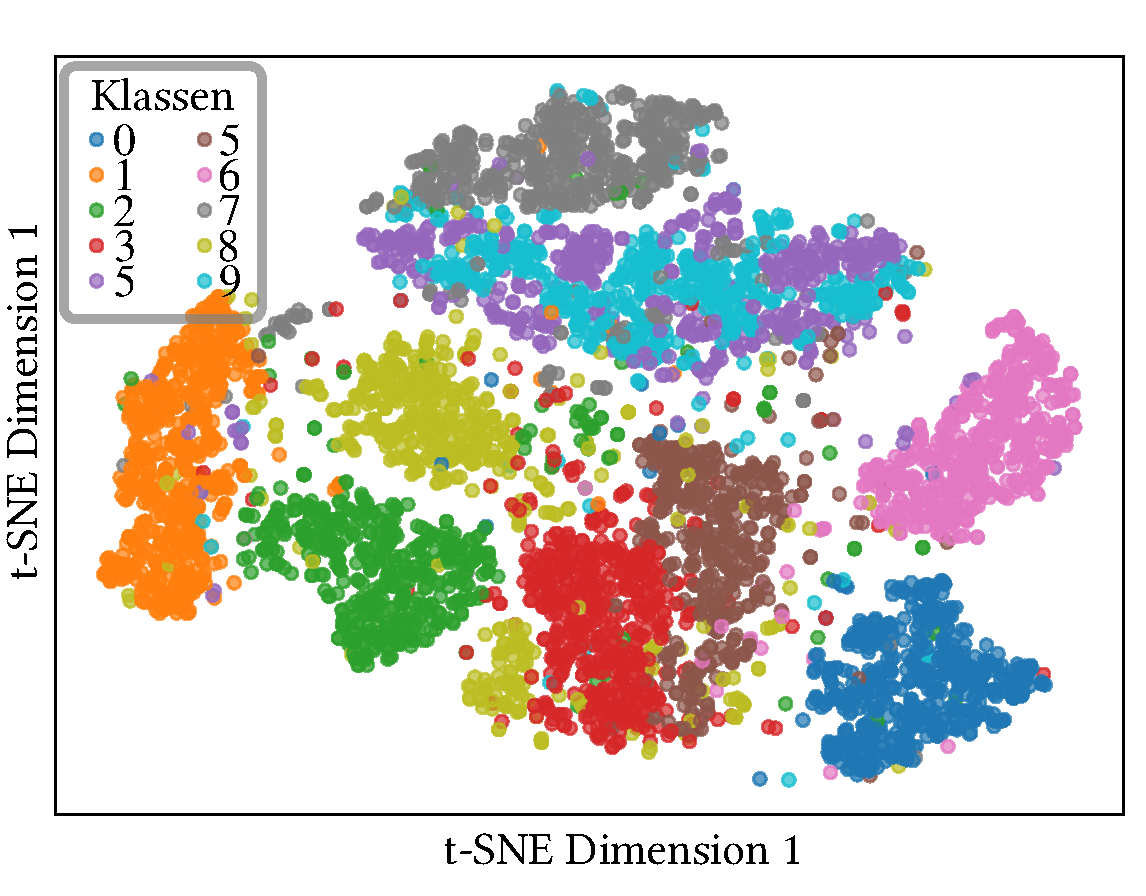
\includegraphics[width=\textwidth]{Figures/scatter_bad.pdf}
    \end{subfigure} 
    %\hspace{0.5cm}
    \begin{subfigure}[b]{0.49\textwidth}
        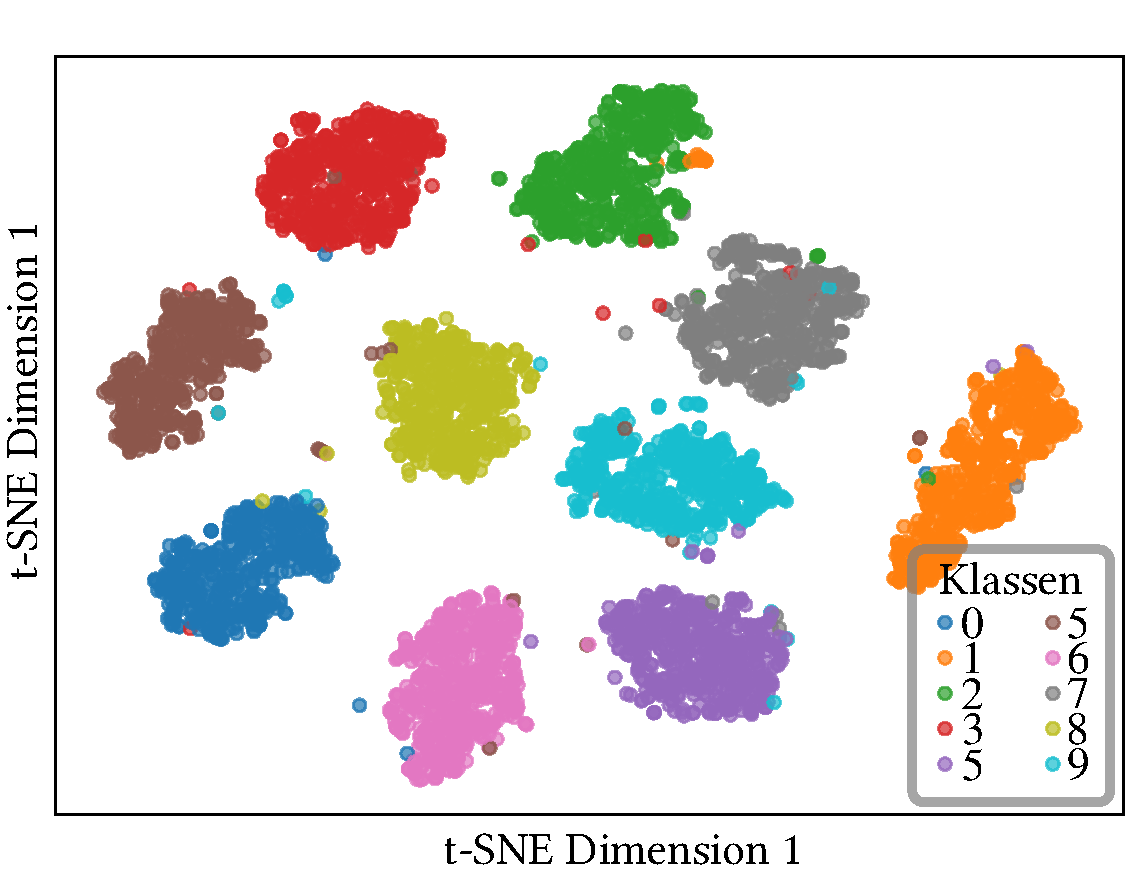
\includegraphics[width=\textwidth]{Figures/scatter_good.pdf}
    \end{subfigure}
    \caption{Zwei Scatterplots.
    Beide Scatterplots visualisieren den Merkmalsraum eines Klassifikators, links nach der ersten Epoche des Trainings, rechts nach 25 Epochen.
    Mithilfe der \ac{tsne} wird die hochdimensionale interne Repräsentation der Merkmale in eine zweidimensionale Ansicht projiziert.
    Einige Stichproben des MNIST-Datensatzes sind in dieser zweidimensionalen Ansicht platziert und ihre Klassen sind farblich markiert.}
    \label{fig:scatter_tsne_example}
\end{figure}
\noindent 
Dreidimensionale Daten stellen eine besondere Herausforderung für die Klassifikation dar \cite{Tran2018}.
Vortrainierte Methoden der 2D-Klassifikation wie \ac{cnn}-Encodern können auf einzelne Schichten eines 3D-Volumens angewandt werden, und die extrahierten Merkmale können anschließend aneinandergereiht werden, aber explizite 3D-Methoden sind oft besser \cite{Feichtenhofer2020}.
Die Methoden können auch an dreidimensionale Daten angepasst werden, indem ihre 2D-Operationen auf drei Dimensionen ausgeweitet werden, wodurch der Rechenaufwand steigt \cite{Carreira2017}.
Angepasste Methoden wie 3D-\acp{cnn} sind nicht in der Lage, Beziehungen zu erfassen, wenn die relevanten Bildregionen räumlich weit voneinander entfernt sind und schräg in den drei Dimensionen verteilt sind \cite{Tran2015}. 
Um dieses Problem zu lösen, schlägt die Literatur self-attention-Mechanismen über die Z-Dimension vor, die auch nicht-lokale Informationen erfassen \cite{Bertasius2021, Wang2018}. 
\section{Literaturrecherche}
\subsection{Benchmark}\label{sec:bench}
Da das Annotieren von Zelldaten für die Segmentierung mit erheblichem manuellen Aufwand verbunden ist und zusätzlich Expertenwissen voraussetzt, sind Datensätze hierfür selten.
Einige prominente Datensätze mit Annotationen für eine Instanzsegmentierung, deren Domänen zu den Zieldaten der Anwendung dieser Arbeit \textit{ähnlich} sind, sind:  
\begin{itemize}
    \item LiveCell \cite{edlund2021livecell}, ein manuell annotierter und von Expert*Innen validierter Datensatz aus 5.239 2D-Bildern. 
    Die Daten sind mit Phasenkontrastmikroskopie gesammelt und enthalten 1.686.352 individuelle Zellen von acht verschiedenen Zelltypen.
    \item YeaZ \cite{dietler2020YeaZ}, ein zweiteiliger Datensatz von Hefe-Zellen aus 87 Phasenkontrast-Bildern mit insgesamt 10.422 Zellen und 614 Hellfeld-Bildern mit insgesamt 3.841 Zellen in 6 Beleuchtungsstufen aufgenommen. Die Annotationen sind semi-manuell erstellt, da die Phasenkontrast-Bilder manuell und die Lichtfeld-Bilder aus den Phasenkonstrast-Segmentierungsmasken annotiert wurden. 
    \item DeepBas \cite{holden2021deepbacs, cspahn2021deepbacs}, ein Datensatz von \textit{B. subtilis strain SH130} Bakterien. Er besteht aus Weitfeldaufnahmen (Fluoreszenz), aufgenommen mit einem inversen Mikroskop, bestehend aus sieben manuell annotierten Bildern mit je 46 bis 335 Zellen.
    \item die Cell Tracking Challenge \cite{ulman2017cellTrackingChallenge}, eine Sammlung aus 13 Datensätzen verschiedener Mikroskopiemodalitäten, die sich zur Messung der Segmentierungs- und Verfolgungsfähigkeiten für verschiedene Zelltypen eignen.
    \item MoNuSeg \cite{kumar2017MoNuSeg}, eine Zusammenstellung manuell annotierter Gewebeschnitte aus sieben verschiedenen Organen. Über 21.000 Zellen sind pro Bild in den 30 Bildern mit verschiedenen Färbungen und Aufnahmetechniken verteilt.
    \item TissueNet \cite{greenwald2022Tissuenet} ist ein umfassender Datensatz mit über 1.000.000 Zellen aus verschiedenen Gewebearten und unterschiedlichen Aufnahmetechniken.
    \item S\_BIAD1518 \cite{Kromp2020_Dataset, chen20223_Dataset}, ein Datensatz, der neben manuell annotierten Bildern von acht verschiedenen Zellarten synthetisch erzeugte Daten enthält. Mithilfe von SpCycleGAN \cite{fu2018cycleGAN} wurden dazu auf Basis simulierter Annotationen Bilder generiert, die anstreben, die Merkmale der realen Bilder zu reproduzieren. Es handelt sich um 3D-Multispektraldaten, aufgenommen mittels Fluoreszenzbildgebung. 
\end{itemize}
Aufgrund des geringen Volumens an frei zugänglichen Daten sind diese Sammlungen auch für das Training von Segmentierungsnetzen begehrt. 
Neben annotierten Datensätzen bietet die Literatur auch Methoden zum eigenständigen Erzeugen domänenspezifischer Datensätze \cite{Abay2019, Raghunathan2021, Nikolenko2021, Choi2017, Lu2023}.
Beispielsweise können 3D-Trainingsdaten mit realistischer Zellform und -ausrichtung sowie umgebenden Markern synthetisch erzeugt und durch ein Generative Adversarial Network an eine gewünschte Bilddomäne angepasst werden \cite{bruch2025}. 

\subsection{Segmentierungsmodelle}
Foundation-Modelle sind für viele moderne \ac{ki}-Anwendungen unerlässlich \cite{bommasani2021foundationmodels}. 
Sie werden zunächst für allgemeine Aufgaben vortrainiert und anschließend auf spezifische Anwendungen angepasst (fine-tuning), meist unter Einfrieren von Teilen der Gewichte \cite{Yosinski2014}.
Auch Segmentierungsmodelle profitieren stark von umfangreichem Vortraining \cite{dippel2022segmentation}. 
In der aktuellen Forschung werden verschiedene Foundation-Modelle zur Segmentierung angewandt \cite{wang2021max,zou2023segment,jain2023oneformer,li2023mask}.
Ein prominentes Exemplar ist das \ac{sam} von Meta AI \cite{kirillov2023sam} (siehe Abb. \ref{fig:SAM_Architektur}). 
Es besteht aus einem Bild-Encoder, einem Prompt-Encoder und einem Masken-Decoder. 
\begin{figure}[H]
    \centering
    \includegraphics[width=1\linewidth]{Figures/SAM_Architecture.png}
    \caption{Architektur des \ac{sam}-Modells. 
    Eingabebilder werden durch einen Bildencoder in Repräsentationen umgewandelt. 
    Zusätzliche optionale Hinweise zum zu segmentierenden Objekt werden durch Bildfaltungen oder einen Prompt-Encoder repräsentiert. 
    Anschließend prädiziert der Decoder mehrere mögliche Masken und die zugehörigen Zuversichtlichkeiten \cite{kirillov2023sam}.}
    \label{fig:SAM_Architektur}
\end{figure}
\noindent
Als Bild-Encoder dient ein Vision Transformer \cite{dosovitskiy2020ViT} mit Vortraining als Masked Autoencoder \cite{he2022mae} und zusätzlichem Training für höhere Bildauflösung.
Der Prompt-Encoder ist mehrstufig.
Ein angelernter Positional Encoder generiert Repräsentationen aus Positions-Nutzereingaben wie Punkten und Boxen.
Für textuelle Prompts wird der Encoder des CLIP-Modells \cite{Radford2021} verwendet.
Außerdem werden Bildfaltungen als Encoder auf Maskeneingaben angewandt.
Mithilfe dieser Encoder wird dem Modell eine Repräsentation des zu segmentierenden Bildes sowie optional Hinweise auf das erwünschte Ergebnis bereitgestellt, die bereits semantische Informationen und abstrakte Bildmerkmale enthalten.
Aus diesen Repräsentationen generiert der Decoder anschließend mehrere mögliche Masken mit zugehörigen Zuversichtlichkeiten, aus denen ein finales Segmentierungsergebnis ausgewählt wird.\\ [0.5\baselineskip]
Das \ac{sam}-Modell wurde bereits für viele explizite Mikroskopie-Zelldaten-Anwendungen angepasst \cite{archit2025samfine, israel2023samfine, vandeloo2025samfine}. 
Auch für bestehende biologische Segmentierungsanwendungen, wie etwa Cellpose\cite{stringer2021cellpose}, wurde \ac{sam} auf Zelldaten angepasst \cite{pachitariu2025samcellpose}.
Dieser \textit{Fine-tune} nennt sich CellposeSAM.
Er kombiniert den Bild-Encoder von \ac{sam} mit dem \linebreak \textit{Flow}-Segmentierungsansatz von Cellpose.
Dabei generiert der Bild-Encoder direkt Vektoren, die Zwischenrepräsentationen, sogenannte \textit{Flows}, darstellen.
Diese \textit{Flows} werden pixelweise zu einem Gradientenfeld überführt.
Mithilfe der Gradienten werden Objektinstanzen vorhergesagt.
Abb. \ref{fig:CellposeSAM} zeigt diesen Ablauf als Diagramm.
\begin{figure}[H]
    \centering
    \includegraphics[width=0.98\linewidth]{Figures/CellposeSAM_Diagramm.png}
    \caption{Ablauf des CellposeSAM-Modells. 
    Eingabebilder werden durch einen Bild-Encoder (ViT-L) direkt zu sogenannten \textit{Flows} umgeformt, einer Repräsentation von vorhergesagten Objektmerkmalen, deren Werte von der relativen Position innerhalb des detektierten Objekts abhängen. 
    Die Gradienten der Flows werden verfolgt (gradient tracking) und aus dem daraus entstehenden Gradientenfeld werden Segmentierungsinstanzen (ROIs) vorhergesagt \cite{pachitariu2025samcellpose}.}
    \label{fig:CellposeSAM}
\end{figure}
\noindent
Deepcell \cite{van2016deepcell,bannon2021deepcell,greenwald2022deepcell} bietet weitere Zellsegmentierungsmodelle.
Das Deepcell-Caliban-Modell \cite{moen2019DeepcellCaliban} nutzt als Encoder eine EfficientNetV2L-Architektur \cite{Tan2021}, an deren Ausgabeschichten eine Pyramidenstruktur zur Merkmalsfusion angeschlossen ist. 
Eine Besonderheit des Netzes ist, dass Eingabebildern zusätzlich Koordinatenkarten hinzugefügt werden.
Als Decoder dienen drei Segmentierungsköpfe, die verschiedene Transformationen der annotierten Trainingsmasken vorhersagen.\\ [0.5\baselineskip]
In der Literatur ist außerdem das nnU-Net \cite{isensee2021nnu} sehr verbreitet, ein Segmentierungsframework, das sich automatisch an neue biomedizinische Aufgaben anpasst.
Es konfiguriert Vorverarbeitung, Netzwerkarchitektur, Training und Nachbearbeitung dynamisch auf Basis der Eigenschaften des jeweiligen Datensatzes. 
Die Leistungsfähigkeit des Ansatzes ergibt sich nicht aus einer neuen Architektur oder einer neuen Lernmethode, sondern aus der konsequenten Automatisierung und Systematisierung von Entwurfsentscheidungen.

\subsection{Klassifikator}
Für Klassifikatoren werden in der Regel nur Encoder vortrainiert.
Der Klassifikations-Kopf muss an die Klassen des vorliegenden Problems angepasst werden \cite{Plested2022, Yosinski2014, Dippel2022}.
State-of-the-Art für Bild-Encoder sind \acp{cnn} oder \acp{vit}, die auf dem ImageNet-Datensatz \cite{Russakovsky2015} vortrainiert werden \cite{You2018, Kornblith2019}.
Klassifikatoren profitieren stark von ImageNet-Vortraining \cite{Beyer2020, Recht2019}.\\[0.5\baselineskip]
\textbf{ResNet} ist ein Residual Neural Network, ein \ac{cnn} mit sogenannten residual connections \cite{He2016}.
Diese residual connections verbinden den Ein- und Ausgang modularer Faltungsschichten und verbessern die Leistungsfähigkeit tiefer neuronaler Netze \cite{He2016, He2015, srivastava2015highway} (siehe Abb. \ref{fig:ResDiagramms} a).
In ihrem Paper stellen die Autoren fünf unterschiedlich tiefe Varianten der \textbf{ResNet}-Architektur vor.
Jede Variante enthält fünf Blöcke mit residual connections.
Die Blöcke bestehen aus Faltungen mit verschiedenen Kernelgrößen und Strides, batch normalization \cite{Ioffe2017} und der ReLU \cite{Nair2010} Aktivierungsfunktion.\\[0.5\baselineskip]
\textbf{EfficientNet V2} ist ein Nachfolger der EfficientNet-Modellfamilie \cite{Tan2021, Tan2019}.
Die Architektur basiert auf modularen Blöcken von Bildfaltungsoperatoren mit besonders kleinen Faltungskernen und Squeeze-and-Excitations, genannt MBConv \cite{Tan2019, Sandler2018} und \linebreak Fused-MBConv \cite{Gupta2019} (siehe Abb. \ref{fig:ResDiagramms} b).\newline
\begin{figure}[H]
    \centering
    \includegraphics[width=0.98\textwidth]{Figures/Convs.pdf}
    \caption{Diagramme a) der Residual Connections \cite{He2016} und b) der MBConv-Blöcke und der Fused-MBConv-Blöcke \cite{Tan2021}.}
    \label{fig:ResDiagramms}
\end{figure}
\noindent
\textbf{ConvNeXt} \cite{Liu2022} ist eine \ac{cnn}-Modellfamilie mit besonders großen Faltungskernen. 
Die \textbf{ConvNeXt}-Architektur umfasst fünf modulare Blöcke mit Faltungen und residual connections, wie die ResNet-Architektur \cite{He2016}.
Allerdings verändert dabei \textbf{ConvNeXt} einige Details der ResNet-Architektur, wie beispielsweise die GeLU-Aktivierungsfunktion \cite{Hendrycks2016} und layer normalization \cite{Ba2016}.\\ [0.5\baselineskip]
Swin Transformer \cite{liu2021} ist eine beliebte Modellfamilie der \acp{vit}.
Ihr Nachfolger, die \textbf{Swin Transformer V2}-Familie \cite{Liu2022a}, vergrößert die Modelle weiter.
Die Architektur kombiniert Bildausschnitte mit einem Positionsbias.
Hierzu werden ein Bildfenster $z$ und dessen relative Koordinaten im Bild, $\Delta x$ und $\Delta y$, in einem attention-Mechanismus zusammengeführt.
Die Positionen werden in einem MLP-Netz verarbeitet, während das Bildfenster mit drei verschiedenen Gewichtsmatrizen multipliziert wird.
Mithilfe einer Kosinusähnlichkeitsfunktion, der Softmax-Funktion \cite{Bridle1989}, der elementweisen Multiplikation sowie der Addition werden diese Ergebnisse in einen Merkmalsraum überführt.
Zwei layer normalizations \cite{Ba2016}, ein weiteres MLP-Netz und residual connections vervollständigen anschließend den modularen \textbf{Swin Transformer V2}-Block.
Dieser Aufbau ist in Abb. \ref{fig:SwinArchitecture} im Anhang dargestellt. 
Der Abschnitt \ref{supp:swin} des Anhangs zeigt die Architektur als Diagramm.
\section{Offene Probleme}
Einzelne Myotuben lassen sich nicht mithilfe eines Segmentierungsmodells aus der Literatur instanzsegmentieren.
Selbst für Expert*Innen sind in dichten Strukturen Myotuben-Instanzen nicht immer eindeutig trennbar.
Nicht viele Segmentierungsmodelle für Nuclei sind erhältlich, insbesondere für dreidimensionale Daten.
Die verfügbaren Modelle verhalten sich je nach Datensatz unterschiedlich, und ihre Eignung für bestimmte Aufgaben muss in jeder Anwendung individuell geprüft werden.
Die Daten der vorliegenden Arbeit wurden gemäß dem Protokoll in Couturier et al. \cite{Couturier2024} erstellt und umfassen Myotubenkulturen sowie deren Nuclei und sind mit insgesamt fünf verschiedenen Fluoreszenzmarkern versehen.
Für diese spezifischen Aufnahmebedingungen und Marker der vorliegenden Daten gibt es keinen angepassten Klassifikator.
Der Erfolg eines Übertrags verschiedener vortrainierter Encoder und etablierter Methoden auf die vorliegenden Daten ist unvorhersehbar, da sich die gelernten Merkmalsräume möglicherweise nicht für die Klassifikation der neuartigen dreidimensionalen Daten eignen.
Eine weitere Fragestellung ist deshalb, wie Klassifikationsmethoden mit der Kombination der Marker umgehen. 
Für jeden Datensatz mit neuen Zellkernklassen und Aufnahmebedingungen muss nicht nur ein neues Modell trainiert, sondern auch Methoden- und Hyperparameteroptimierung durchgeführt werden, um optimale Klassifikatorleistung zu erzielen.
Des Weiteren ist der Umgang mit dreidimensionalen Daten, insbesondere in Umgebungen mit geringer Rechenleistung, ein offenes Problem.
Diverse Lösungen existieren, um dreidimensionale Daten mit Expertenwissen zu versehen.
Diesen Lösungen fehlt bislang ein Arbeitsablauf, der Daten unmittelbar segmentiert und vorbereitet, um relevante Bildausschnitte direkt aus dem Datensatz zu extrahieren, sodass Expert*Innen ausschließlich annotieren müssen.
\newpage
\section{Zielsetzung}
Im Zuge der vorliegenden Arbeit soll die automatische Extraktion interpretierbarer Eigenschaften der Myotubenkulturen ermöglicht werden.
Zu diesem Ziel definiert die vorliegende Arbeit folgende Zwischenziele:
\begin{itemize}
    \item Es soll ein Segmentierungsmodell gefunden werden, das die Eigenschaften wie Zellkernvolumina und die lokale Nucleidichte möglichst unverändert aus den vorliegenden, dreidimensionalen Daten extrahieren kann.
    Dazu wird ein neues Bewertungskriterium für die Instanzsegmentierung eingeführt und auf einige etablierte Modelle angewandt.
    \item Das Segmentierungsmodell soll dann genutzt werden, um einen Ablauf zu schaffen, in dem Expert*Innen die Klassen der Nuclei besonders zeiteffizient annotieren können, um einen Klassifikator zu trainieren.
    Durch das Anreichern dreidimensionaler Daten mit den Segmentierungsmasken und das automatische Fokussieren einzelner Nuclei sollen sowohl die Rechenzeit optimiert werden als auch der Aufwand, einzelne Nuclei entlang drei Dimensionen zu suchen, eliminiert werden.
    Hierzu wird eine neue Anwendung entwickelt, die 3D-Zelldaten liest und anschließend eine Oberfläche zur Annotierung bereitstellt.
    \item Die entstehenden Annotationen sollen direkt in einen Trainingsablauf für Klassifikatoren integriert werden.
    Hierbei müssen Klassifikatoren mit dreidimensionalen Daten variabler Tiefe umgehen können.
    Ein ausführlicher Methodenvergleich verschiedener Encoder, Klassifikations-Köpfe, Vorverarbeitungsmethoden sowie Vortrainingsmethoden soll für Nutzer*Innen ohne Programmierkenntnisse ermöglicht werden.
    Dazu wird eine neue Anwendung entwickelt, die die erstellten Annotationen und Segmentierungsmasken nutzt, um einen Klassifikator zu trainieren.
    Nutzer*Innen können in einer grafischen Oberfläche verschiedene Methoden zum Vergleich auswählen, und in einem automatisierten Prozess werden Klassifikatoren aller Kombinationen trainiert und verglichen.
    \item Außerdem sollen die ausgelesenen Eigenschaften der eingegebenen Zelldaten leicht zugänglich sein.
    In einer weiteren neuen Anwendung werden automatisch die Vorhersagen des Klassifikators mit dem besten Ergebnis im Methodenvergleich genutzt, um Nutzer*Innen Graphen mit den Eigenschaften der Zellkultur darzubieten.
    \item Zuletzt sollen alle neu entwickelten Module zu einer Gesamtanwendung zusammengefasst und getestet werden.
    In einer Parameterbestimmung wird das Optimum für die vorliegenden Aufnahmen explizit mithilfe der neuen Anwendung bestimmt.
\end{itemize}
% !TeX root = ../Thesis.tex

\chapter{Neues Konzept} \label{ch:NewMethods}
\section{Überblick}
Das nachfolgende Kapitel beschreibt und diskutiert im Detail das angewandte Konzept der vorliegenden Thesis. 
Es behandelt die selbstentwickelten Beiträge zu den Methoden sowie die vorliegenden dreidimensionalen Bildstapel der Myotuben-Zellkulturen.
Auf die in Abschnitt \ref{sec:daten} beschriebenen Daten werden die eingeführten Methoden angewandt, um deren Effektivität zu demonstrieren.
In Abschnitt \ref{sec:Kriterien} wird ein neues Bewertungskriterium für 3D-Instanzsegmentierungsmodelle eingeführt.
Es bewertet Modelle im Hinblick auf ihre Eignung, interpretierbare Merkmale von Nuclei unverändert zu extrahieren.
Abschnitt \ref{sec:MethodsClassifier} führt Methoden zur Klassifikation von 3D-Daten ein.
Diese Methoden passen den Klassifikator an verschiedene Eigenschaften eines Datensatzes an.\\[0.5\baselineskip]
Die gesamte Methodik wird in einer modularen Anwendung umgesetzt, die 3D-Daten als Eingabe annimmt und interpretierbare Eigenschaften, wie die Verteilung der Klassen und das Volumen der anwesenden Nuclei, ausgibt.
Diese Anwendung wird hier als 3D-Zelldaten-Pipeline bezeichnet.
Abb. \ref{fig:graph_abstract} bietet einen Überblick über die Methodik.
Die Anwendung kann regulär angewandt (Inferenz) oder optimiert werden (Optimierung).
Zur Optimierung werden die 3D-Daten einem Ablauf für den Vergleich der Segmentierungsmodelle oder der Klassifikatormethoden zur Verfügung gestellt.
Zuerst wird das neu eingeführte Bewertungskriterium für Segmentierungsmodelle \acf{ipq} für verschiedene Modelle berechnet (siehe Kapitel \ref{sec:Kriterien}).
Dieses Bewertungskriterium quantifiziert die Eignung der Segmentierungsmodelle zur Extraktion der gewünschten Zellkerneigenschaften.
Mithilfe der \ac{ipq}-Werte wird das beste Segmentierungsmodell für die Anwendung gewählt.
Die Architektur und Parameter des optimalen Modells werden in den Inferenzablauf eingesetzt.\\[0.5\baselineskip]
Um die Klassifikatormethoden zu optimieren, werden die 3D-Daten und die extrahierten Segmente in die neu entwickelte Labeling-App eingegeben.
Die Labeling-App ermöglicht die zeiteffiziente Annotation von Nuclei, indem relevante Bildausschnitte automatisch anhand der Segmente extrahiert werden.
Mit den erstellten Annotationen und den 3D-Daten werden iterativ verschiedene Klassifikatoren trainiert.
Diese Klassifikatoren ergeben sich aus Kombinationen der verfügbaren Klassifikatormethoden.
Die Klassifikatormethoden werden in Kapitel \ref{sec:MethodsClassifier} beschrieben und umfassen 1. Encoder-Architekturen, 2. Klassifikations-Kopf-Architekturen, 3. Vorverarbeitungsmethoden und 4. Vortrainingsmethoden.
Unter den Methoden sind sowohl etablierte als auch neu entwickelte Ansätze.
Anhand der Genauigkeit der trainierten Klassifikatoren auf einem separaten Validierungsanteil des Datensatzes werden die Methoden verglichen und eine optimale Konfiguration ausgegeben.
Die Architektur und Parameter dieser Konfiguration werden dann in den Inferenzablauf der Anwendung eingesetzt.\\[0.5\baselineskip]
Am Ende des Ablaufs werden die klassifizierten Segmente verwendet, um verschiedene Grafiken zu erzeugen, die interpretierbare Eigenschaften visualisieren.
\begin{figure}[h]
  \centering
  \includegraphics[width=0.99\linewidth]{Figures/graphAbstract_flowchart.pdf}
  \caption{Methodik der vorliegenden Arbeit.
  Die Anwendung kann regulär angewandt (Inferenz) oder optimiert werden (Optimierung).
  Die Optimierung ist zweiteilig.
  Zur Optimierung der Segmentierungsmodelle wird das neu entwickelte \acf{ipq}-Bewertungskriterium eingesetzt.
  Für den Klassifikator werden Kombinationen verschiedener Encoder, Klassifikations-Köpfe, Vorverarbeitungsmethoden und Vortrainingsmethoden iterativ trainiert und verglichen. 
  }
  \label{fig:graph_abstract}
\end{figure}
\noindent

\section{Daten}\label{sec:daten}
Die zugrunde liegenden Bilddaten der vorliegenden Arbeit stammen aus in-vitro-Kulturen von Myotuben, die aus humanen induzierten pluripotenten Stammzellen (hiPSC) differenziert wurden. 
Diese Zellen wurden nach dem in Couturier et al. \cite{Couturier2024} beschriebenen Protokoll hergestellt und anschließend mittels Immunfluoreszenzfärbung markiert. 
Von den Zellen wurden 3D-Bildstapel mit voxelbasierten Intensitätswerten, die jeweils einem Fluoreszenzkanal zugeordnet sind, mit einem Konfokalmikroskop aufgenommen.
Die Kulturen enthalten Myotuben und deren Nuclei in fünf Fluoreszenzkanälen, die entsprechend mit fünf unterschiedlichen Fluoreszenzmarkern angefärbt wurden:
\begin{itemize}
  \item DAPI (Nuclei),
  \item $\alpha$-Actinin (sarcomerisches Strukturprotein),
  \item Dystrophin (Membran-assoziiertes Muskelprotein),
  \item Synaptophysin (präsynaptisches Vesikelprotein),
  \item $\alpha$-Bungarotoxin (Bindung an nikotinische Acetylcholinrezeptoren, nAChR) und
  \item S100$\beta$ (Schwannzellmarker).
\end{itemize}
Jeder dieser Marker färbt einen anderen Zellbestandteil an, sodass unter dem Mikroskop sichtbar ist, wo sich Kerne, Muskelfasern und synaptische Strukturen befinden.
Die Bildaufnahme erfolgte mit einem Leica TCS SP8 Konfokalmikroskop, unter Verwendung von 405-nm-, 488-nm-, 561-nm- und 633-nm-Lasern und einem 20x-Objektiv. 
Je Kanal ergibt sich eine räumliche Auflösung von 1024 x 1024 Pixeln mit 568 nm pro Pixel.
Die Anzahl der Z-Schichten beträgt 24 bis 64.
Die Proben wurden in Matrigel eingebettet und unter physiologisch relevanten Kulturbedingungen (37 °C, 5\% CO₂) im maturierenden Medium kultiviert, das u. a. Wachstums- und Differenzierungsfaktoren wie BDNF, GDNF, IGF-1, CHIR99021, DMH1, SB431542, Retinsäure und Purmorphamin enthielt.
Das resultierende Material stellt ein menschliches in-vitro-Modell der neuromuskulären Verbindung dar.
Abb. \ref{fig:channel_examples} zeigt exemplarisch je eine 2D-Schicht von einem der Marker-Kanäle.
\begin{figure}[H]
  \centering
  \includegraphics[width=0.9\linewidth]{Figures/channel_examples.pdf}
  \caption{Beispiele von 2D-Schnitten der verfügbaren Färbungen der vorliegenden 3D-Bildstapel.
  }
  \label{fig:channel_examples}
\end{figure}
\noindent
Die eingeführten Methoden werden als Experiment auf diese Daten angewandt, sie sind aber explizit entworfen, um Anpassungen an neue Datensätze nahtlos zu ermöglichen.
Alle Experimente auf diesen Daten dienen der vorliegenden Arbeit als Fallstudie, um die Effektivität der vorgestellten Methoden zu demonstrieren.
\section{Neues Kriterium: Injektive Panoptische Qualität}\label{sec:Kriterien}
Zur Wahl des Segmentierungsmodells wird das neue Bewertungskriterium \acf{ipq} eingeführt.
Es besteht aus drei Faktoren, die jeweils eine Fehlerart bei Instanzsegmentierungsmasken prüfen.
\begin{figure}[h]
  \centering
  \includegraphics[width=0.99\linewidth]{Figures/IPQ_horizontal.pdf}
  \caption{\ac{ipq} Visualisierung - Das Ablaufdiagramm stellt den Prozess dar, durch den das Segmentierungsmodell gewählt wird, das für die Anwendung der vorliegenden Arbeit eingesetzt wird. 
  Ein peer-reviewed Benchmark-Datensatz aus dreidimensionalen Bildern (1) von diversen Zellkulturen mit den dazugehörigen Annotationen wird links eingegeben. 
  Das zu bewertende Segmentierungsmodell (2) führt für die Bilder des Benchmarks eine Inferenz durch, um Segmentierungsmasken (3) bereitzustellen. 
  Die entstehenden Masken werden anschließend zur Berechnung der neu eingeführten \ac{ipq} (siehe Kapitel \ref{sec:Kriterien}) eingesetzt. 
  Der Ablauf der Bewertung ist in drei Phasen gegliedert.
  Aus jeder Maske werden zuerst die einzelnen Fragmente extrahiert, die sich mit einer einzelnen Instanz der Annotation überlagern (4).
  Außerdem wird ein Fehlerbild durch Berechnung der \acf{iou} hergestellt, hier als logische XOR-Fläche der Maske und der Annotation als Platzhalter dargestellt (5).
  Zuletzt wird ein Zuweisungsbild erstellt, das die \acp{tp}, \acp{fp} und \acp{fn} festhält (6).
  Aus diesen drei Teilen wird jeweils ein Faktor zur Berechnung der \ac{ipq} gebildet.
  Durch Vergleiche der Ergebnisse verschiedener Modelle lässt sich dann das optimale Segmentierungsmodell für die Anwendung wählen.}
  \label{fig:ipq}
\end{figure}
\noindent
Als Datensatz wird aus den in Kapitel \ref{sec:bench} vorgestellten Benchmarks der S\_BIAD1518-Datensatz \cite{Kromp2020_Dataset, chen20223_Dataset} verwendet, da dieser nicht in den Trainingsdaten eines zu testenden Segmentierungsmodells vorkommt.
Der Datensatz verfügt über manuelle Annotationen für Instanzsegmentierungsmasken und ist durch synthetisch generierte Daten und Masken erweitert.
Im Gegensatz zu selbstentwickelten synthetischen Daten weicht die Bilddomäne dieses Benchmarks zwar stärker von der Domäne der Zieldaten ab, aber dafür sind die Daten an eine Veröffentlichung mit standardisiertem Peer-Review-Prozess gebunden.\\ [0.5\baselineskip]
Die Aufgabe des Bewertungskriteriums ist es, zu quantifizieren, wie gut sich eine vorliegende Instanzsegmentierung eignet, um reale Eigenschaften einer Aufnahme, wie die Zellkernanzahl, die Größe der Zellkerne und die lokale Zellkerndichte auszuwerten. 
Das neu entwickelte Kriterium ist eine Erweiterung der \ac{pq} \cite{kirillov2019PQ}. 
Durch die \ac{pq} wird die \ac{iou} für individuelle Instanzen bewertet und es werden \ac{fp} sowie \ac{fn} Detektionen bestraft. 
Zusätzlich werden durch einen neuen Faktor Verletzungen der injektiven Abbildung von segmentierten Nuclei auf die Instanzen der Annotation negativ bewertet werden, da die genaue Anzahl der Nuclei und die räumliche Dichte der Nuclei eine bedeutungsvolle Metrik für die Auswertung sind. 
Zur Berechnung wird im ersten Schritt der folgende Brute-Force-Algorithmus angewandt, der die Zuordnung von Segmentierungsinstanzen zu Annotationsinstanzen durchführt.

\begin{algorithm}
\caption{Brute-Force-Annotation-Zuordnung für jede Segmentierungsinstanz}
\begin{algorithmic}
\REQUIRE $maske_\text{Vorhersage}$, $maske_\text{Annotation}$
\ENSURE $annotation_\text{opt}$, $IoU_\text{opt}$

\FOR{$id_\text{Instanz}$ in $|maske_\text{Vorhersage}|$}
  \STATE $Instanz \gets maske_\text{prediction}[id_\text{Instanz}]$

  \FOR{$annotation$ in $maske_\text{Annotation}$}
     \STATE $IoU \gets IoU(annotation, Instanz)$

    \IF{$IoU > IoU_\text{opt}[id_\text{Instanz}]$}
      \STATE $IoU_\text{opt}[id_\text{Instanz}] \gets iou$
      \STATE $annotation_\text{opt}[id_\text{Instanz}] \gets annotation\_id$
    \ENDIF
  \ENDFOR
\ENDFOR

\RETURN $annotation_\text{opt}$, $IoU_\text{opt}$
\end{algorithmic}
\end{algorithm}
\noindent
Die nachfolgende Formel zeigt das \ac{ipq}-Bewertungskriterium unterteilt in die 3 Faktoren \ac{sq}, \ac{rq} und die neu eingeführte \ac{iq}:
\begin{equation}
\text{IPQ} = 
\underbrace{
\frac{k_1 \times \displaystyle\sum_{(p, g) \in TP} 
\text{IoU}\left(\displaystyle\bigcup_{p_i \in p} p_i,\, g\right)
}{|TP|}
}_{\text{Segmentation-Quality (SQ)}}
\times
\underbrace{
\frac{k_2\times|TP|}{|TP| + \frac{1}{2}|FP| + \frac{1}{2}|FN|}
}_{\text{Recognition-Quality (RQ)}}
\times
\underbrace{
\frac{k_3\times\displaystyle |GT|}{\displaystyle\sum_{p \in P} \left( \max(1, n_p - 1) \right)} }_{\text{Injective-Quality (IQ) (neu)}},
\end{equation}\label{eq:ipq}
wobei:
\begin{itemize}
    \item $k_1, k_2, k_3$ Optionale Vorfaktoren zur Gewichtung der drei Teile der Metrik sind,
    \item $TP$ die Menge aller \ac{tp}-Tupel $(p, g)$ ist, wobei $g$ eine Annotationensinstanz und $p$ der Vektor aller zugehörigen Segmentierungsinstanzen ist,
    \item $|TP| \in \mathbb{Z}$ die Anzahl der korrekt erkannten Instanzen bezeichnet, also Annotationsinstanzen mit $\text{IoU} > 0{,}5$,
    \item \ac{iou}$(\bigcup_{p_i \in p}p_i, g) \in [0,1] $ die \ac{iou} zwischen allen Segmentierungsinstanzen $p_i$ in der \ac{tp}-Instanz \textit{p} und der zugehörigen Annotationsinstanz \textit{g} beschreibt,
    \item $|FP| \in \mathbb{Z}$ die Anzahl der falsch-positiven Segmentierungen ist, d.\,h. vorhergesagte Instanzen ohne Annotationsentsprechung,
    \item $|FP| \in \mathbb{Z}$ die Anzahl der nicht erkannten Annotationsinstanzen ist, also Annotationsinstanzen ohne zugehörige Vorhersage,
    \item $|GT| \in \mathbb{Z}$ die Anzahl der Annotationsinstanzen ist,
    \item $P$ die Menge aller Segmentierungsinstanzen ist, ungeachtet der Annotationszuordnung,
    \item $p \subseteq P$ ein Vektor aller Segmentierungsinstanzen, die der gleichen Annotationsinstanz zugeordnet sind, ist,
    \item $n_p$ die Dimension des Vektors $p$ ist,
    \item $\text{SQ} \in [0,1]$ ein Faktor ist, der die Qualität der Segmentierung anhand der \ac{iou} von der segmentierten und der erwarteten Instanz vergleicht,
    \item $\text{RQ} \in [0,1]$ ein Faktor ist, der bewertet, wie vollständig und fehlerfrei das Segmentierungsmodell die vorhandenen Nuclei findet und, ob es dabei zu Halluzinationen kam,
    \item $\text{IQ} \in [0,1]$ ein Faktor ist, der das Unterteilen von Nuclei durch das Segmentierungsmodell zu bestrafen. Wird ein Nucleus durch mehrere Instanzen der Segmentierungsmaske dargestellt, wird $n_p$ größer als eins und der Faktor sinkt,
    \item $\text{IPQ} \in [0,1]$ ein Maß für die panoptische Segmentierungsqualität mit der Voraussetzung von injektiver Abbildung der Segmentierungsmasken-Instanzen auf die Annotationsinstanzen darstellt, wobei höhere Werte bessere Übereinstimmung bedeuten,
\end{itemize}
\noindent
Der \ac{sq}-Faktor bestraft Fehler, die das Volumen von Nuclei verändern, mit dem \ac{rq}-Faktor werden Veränderungen der Zellkernanzahl bestraft und der \ac{iq}-Faktor bestraft Veränderungen der lokalen Zellkerndicht. \newpage
\section{Klassifikatormethoden}\label{sec:MethodsClassifier}
\subsection{Übersicht}
Jedem instanzsegmentierten Nucleus wird eine Klasse zugewiesen, um die Ausgabe zur panoptischen Segmentierungsmaske zu erweitern.
Erst die panoptische Segmentierungsmaske ermöglicht das automatische Extrahieren interpretierbarer Eigenschaften aus den Daten.
Durch diese panoptische Maske und die extrahierten Eigenschaften der Myotuben-Kultur wird ein klarer Überblick über den aktuellen Stand der Zellkultur geboten.\\ [0.5\baselineskip]
Für die Klassenzuweisung ist ein Klassifikator notwendig, der einen Bildausschnitt mit einer Nucleus-Instanz als Eingabe annimmt und eine Klasse als Ausgabe ausgibt.
Um diesen Klassifikator optimal zu entwerfen, wird ein umfangreicher Benchmark aus den Zieldaten erstellt, mit dem die vorgestellten Methoden verglichen werden.
Benchmarks aus der Literatur umfassen weder dieselben Klassen noch dieselben Objektmerkmale.
Deshalb wird ein eigener, kein etablierter Benchmark verwendet.
Für das Training wird einheitlich der Adam-Algorithmus \cite{Kinga2015} mit einer Lernrate von 0,0001 eingesetzt.
Außerdem wird der Cross-Entropy-Loss \cite{Sukhbaatar2014} verwendet. \\ [0.5\baselineskip]
Aus den annotierten Bilddaten werden für jede Anwendung ein Test- und ein Trainingsanteil im Verhältnis eins zu neun extrahiert.
Alle betrachteten Variationen des Klassifikators werden ausschließlich mit den Trainingsdaten trainiert und ihre Leistung ausschließlich anhand der Testdaten getestet.
Beide Anteile des Datensatzes werden durch Augmentierung erweitert und anschließend in Batches zusammengefasst.
Zur Datenaugmentierung werden die folgenden Methoden eingesetzt:
\begin{itemize}
  \item \textbf{Rotation:} Mit einer Wahrscheinlichkeit von 50\% werden die Eingabedaten um 90° in der XY-Ebene rotiert.
  \item \textbf{Spiegelung:} Ebenfalls mit einer Wahrscheinlichkeit von 50\% erfolgt eine Spiegelung entlang der Z-Achse.
  \item \textbf{Gaußsches Rauschen:} Mit einer Wahrscheinlichkeit von 20\% wird Rauschen mit einem Mittelwert von 0 und einer Standardabweichung von 0{,}01 hinzugefügt.
\end{itemize}
Prominente Encoder aus der Literatur werden vergleichend eingesetzt. 
Darüber hinaus werden hier verschiedene Methoden der Vorverarbeitung, des Vortraining und der \linebreak Klassifikations-Kopf-Architektur eingeführt.\\[0.5\baselineskip]
Im Folgenden sind diese Methoden einzeln beschrieben.
Da jede mögliche Kombination mit jedem Netz zu trainieren einen unausführbar hohen Rechenaufwand bedeutet, wird eine Vorauswahl von Kombinationen getroffen. 
\newpage
\subsection{Encoder}
Insgesamt sechs verschiedene Bild-Encoder werden für den Methodenvergleich eingesetzt. 
Tab. \ref{tab:network_comparison} zeigt diese sechs Encoder.
\begin{table}[H]
  \centering
  \caption{Vergleich der sechs vortrainierten Modelle, deren Encoder für den Methodenvergleich eingesetzt werden, hinsichtlich ihrer Genauigkeit auf dem ImageNet-Datensatz \cite{Russakovsky2015} und ihrer Parameter.
  Angegeben sind sowohl die Top-1-Genauigkeit (Acc@1) als auch die Top-5-Genauigkeit (Acc@5), also  ob die korrekte Klasse die zuversichtlichste Vorhersage, bzw. unter den fünf zuversichtlichen Vorhersagen ist.}
  \label{tab:network_comparison}
  \begin{tabular}{lccc}
    \hline
    \textbf{Name} & \textbf{Acc@1 (ImageNet)} & \textbf{Acc@5 (ImageNet)} & \textbf{Parameter (Mio)} \\
    \hline
    ResNet18	      & 69.76\%	& 89.08\% &	11.7 \\
    ResNet101	      & 77.37\%	& 93.55\% &	44.5 \\
    Swin V2	        & 84.11\%	& 96.87\% &	87.9 \\
    ConvNeXt	      & 84.41\%	& 96.98\% &	197.8 \\
    EfficientNet V2 &	85.81\%	& 97.79\% &	118.5 \\
    CellposeSAM	    & -       &	-       &	305 \\
    \hline
  \end{tabular}
\end{table}
\noindent  
In der Tabelle sind die Namen, die Anzahl der Parameter und, falls vorhanden, die Top-1-Genauigkeit (Acc@1) und die Top-5-Genauigkeit (Acc@5) auf dem ImageNet-Datensatz angegeben.
Bis auf das Segmentierungsmodell CellposeSAM handelt es sich um Encoder, die aus Klassifikatoren stammen, die auf dem ImageNet-Datensatz \cite{Russakovsky2015} vortrainiert sind.
Swin V2 und der CellposeSAM-Encoder sind \ac{vit}-Architekturen, während die anderen Encoder \acp{cnn} sind.
\subsection{Vorverarbeitung}\label{sec:Preproc}
Da sich in vielen Bildausschnitten zwei oder mehr Nuclei überschneiden, werden zwei Vorverarbeitungsmethoden eingeführt, die dem Klassifikator signalisieren, welcher der sichtbaren Nuclei klassifiziert werden soll.
Diese Methoden unterscheiden sich darin, wie die Segmentierungsmaske des Nucleus dem Klassifikator zugänglich gemacht wird.
Die erste Methode, hier Masken-Methode genannt, ersetzt den Nucleus-Kanal durch die Segmentierungsmaske des gesuchten Nucleus.
Das Ziel ist, das Risiko zu minimieren, dass umliegende Nuclei das Klassifikationsergebnis verfälschen.
Die Klassifikationsentscheidung wird mit der Masken-Methode von der Geometrie des Nucleus abhängig gemacht.
Mit der Methode geht ein Verlust der Oberflächenmerkmale einher.
Außerdem hängt das Klassifikationsergebnis bei dieser Vorverarbeitungsart stärker von der Qualität der Segmentierung ab.
Ein Erfolg der Methode weist auf einen hohen Informationsgehalt in der Geometrie hin.\\[0.5\baselineskip]
Die zweite Methode wird hier Distanz-Methode genannt.
Mit der Distanz-Methode wird der Nucleus-Kanal mit einer Entfernungsmaske gewichtet.
Hierzu wird pixelweise der originale Nucleus-Kanal mit einer Transformation des Abstands aller Pixel außerhalb der Segmentierungsmaske wie folgt multipliziert:
\begin{equation}
I'(x) = I(x) \cdot \exp\left( -\frac{1}{\sigma} \min_{y \in \lnot M} \|x - y\|_2 \right),
\label{eq:distance}
\end{equation}
wobei:
\begin{itemize}
  \item $\quad I(x) \in [0, 1]$ der Intensitätswert des Nucleus-Kanal an der Position $x$ ist,
  \item $\quad I'(x)  \in [0, 1]$ der Intensitätswert des neuen, transformierten Nucleus-Kanal an der Position $x$ ist,
  \item $\quad x \in \Omega \subset \mathbb{N}^3$ die Position eines Voxels im diskreten Bildraum ist,
  \item $\quad M \subseteq \Omega$ die Segmentierungsmaske und $\lnot M = \Omega \setminus M$ deren Komplement im Bildraum sind,
  \item und $\sigma \in \mathbb{R}^+$ ein Parameter zur Steuerung des exponentiellen Abfalls ist.
\end{itemize}
Die Verwendung der Distanz-Methode hat zum Ziel, die Oberflächenmerkmale des Nucleus zu erhalten.
Außerdem wird mit der Vorverarbeitungsmethode der Einfluss eventuell fehlerhafter Segmentierungsmasken durch die kontinuierliche Abstandstransformation minimiert.
Allerdings ist hierdurch auch das Risiko einer Einflussnahme auf das Klassifikationsergebnis durch umliegende Nuclei nicht vollständig eliminiert, sondern nur vermindert.
In Abb. \ref{fig:preproc_methods} sind die Nucleus-Kanäle der verschiedenen Methoden und die Entfernungsmaske dargestellt.
\begin{figure}[H]
  \centering
    \includegraphics[width=0.98\linewidth]{Figures/preproc.pdf}
  \caption{2D-Schnitte aus ausgeschnittenen 3D-Bildbereichen zur Darstellung der beiden Vorverarbeitungsmethoden. 
  a) Ausgeschnittener Bereich des originalen Nucleus-Kanals mit mehreren, intuitiv trennbaren Nuclei.
  b) Segmentierungsmaske des Nucleus.
      Die Masken-Methode ersetzt den originalen Nucleus-Kanal durch diese Maske.
      Die binäre Maske zeigt keine Oberflächenmerkmale des Nucleus, lediglich geometrische Merkmale.
  c) Entfernungsmaske des Nucleus. 
      Diese wird pixelweise mit dem Nucleus-Kanal für die Distanz-Methode multipliziert.
  d) Mit der Entfernungsmaske gewichtetes Original. Diese Darstellung wird mit der Distanz-Methode an den Klassifikator übergeben.
      Zu sehen ist, dass der nahegelegene ungewünschte Nucleus noch stellenweise mit hoher Intensität vorhanden ist.
  }
  \label{fig:preproc_methods}
\end{figure}
\noindent
Je nach Modellarchitektur müssen die Bilddaten noch skaliert werden, bevor sie den vortrainierten Modellen übergeben werden können, da die Klassifikatoren Eingaben konstanter Größe benötigen.
Dazu wird einfache bilineare Interpolation verwendet (siehe Kap. \ref{sec:Klassifikation}). 
Um Einfluss auf die Ergebnisse durch eine ungleichmäßige Verteilung der Annotationen auf die vorhandenen Klassen zu vermeiden, wird vor dem Training die Anzahl der Stichproben pro Klasse extrahiert.
Mithilfe der Anzahlverteilung werden die Gradienten dann stärker gewichtet, die zu unterrepräsentierten Klassen gehören.
Weil hier mit rechenzeitintensiven dreidimensionalen Daten umgegangen werden muss, ist auch ein dynamisches Speichermanagement Teil der Vorverarbeitungsmethoden. 
Die Anwendung aller beschriebenen Vorverarbeitungsmethoden wird in einem neu entwickelten 'Retreiver' zusammengefasst.
Dieser Retreiver extrahiert die aktuell gewünschten Bildausschnitte, wendet die Vorverarbeitungsmethoden an, zählt die Stichproben pro Klasse und verschiebt nur die notwendigen Daten auf die GPU.
\subsection{Vortraining}\label{sec:Pretrain}
Aus der Literatur sind verschiedene Methoden des Vortrainings bekannt.
Hier werden:
\begin{itemize}
  \item kein Vortraining,
  \item semi-supervised, und
  \item fully-supervised Vortraining 
\end{itemize}
betrachtet.
Die Abb. \ref{fig:pretrain} zeigt die hier umgesetzten Methoden.
\begin{figure}[h]
  \centering
  \includegraphics[width=0.98\linewidth]{Figures/PretrainingMethods.png}
  \caption{Übersicht über die Vortrainingsmethoden. 
  Links zu sehen sind die beiden verfügbaren Bildermengen, ImageNet und die Zieldaten.
  Rechts von diesen Bildermengen werden den Bildern Annotationen hinzugefügt, entweder durch die ImageNet-Datenbank, Expert*Innen oder einen Algorithmus.
  Jeder Encoder (linke Seite eines Netzwerks) und jeder Klassifikations-Kopf (rechte Seite eines Netzwerks) werden mit einer dieser drei Annotationsmengen trainiert.
  Die Farben der Annotation und des Netzwerks zeigen dabei die Zuordnung.
  Mit offenen oder geschlossenen Schlössern über den Encodern und Klassifikations-Köpfen ist dargestellt, ob die Gewichte eingefroren werden.
  Vier verschiedene Versionen jedes Klassifikators werden hier trainiert.
  Das erste Netzwerk wird auf den ImageNet-Daten vortrainiert. 
  Anschließend wird mit Expert*Innen-Annotationen der Klassifikations-Kopf neu trainiert.
  Das Zweite erhält kein Vortraining; es ist komplett mit den Zieldaten trainiert.
  Für das dritte Netzwerk werden lediglich die Annotationen des semi-supervised Algorithmus eingesetzt.
  Die letzte Variante wird semi-supervised vortrainiert und anschließend mit den Zieldaten fine-tuned. }
  \label{fig:pretrain}
\end{figure}
\paragraph{Kein Vortraining}
Ohne Vortraining startet der Encoder, der den Großteil der Gewichte umfasst, mit zufällig initialisierten Gewichtswerten.
Da diese zufälligen Werte keine sinnvollen Merkmale extrahieren, wird ein besonders langes Training mit den Zieldaten durchgeführt.
Jedes Modell wird jeweils für 75 Epochen trainiert.
 
\paragraph{Semi supervised}
Die semi-supervised Annotationen werden mithilfe eines few-shot-gestützten Cluster-Algorithmus erstellt, der hier als Pseudo-Labler bezeichnet wird.
Ein*e Expert*In erstellt hierzu Annotationen von wenigen Nuclei.
Danach werden aus den restlichen Segmentierungsmasken einige Merkmale extrahiert und zu einem Vektor zusammengefasst.
Zuerst werden das Volumen, die Oberfläche und die Achsenlängen jedes Nucleus direkt bestimmt. 
Außerdem wird die Exzentrizität aus dem Verhältnis der längsten und der kürzesten Achse berechnet.
Für die Kompaktheit wird das Volumen der Maske durch die kleinste mögliche Begrenzungsbox geteilt.
Darüber hinaus wird aus der Z-Schicht, in der die Segmentierungsmaske am größten ist, die 2D-Kontur erfasst.
Aus dieser Kontur wird eine komplexe Zahlenfolge berechnet und der Absolutwert der ersten zehn Koeffizienten als einzelne weitere Merkmale dem Merkmalsvektor hinzugefügt (siehe Abschnitt \ref{sec:Klassifikation}). \\[0.5\baselineskip]
Der Pseudo-Labler normalisiert die Werte der Merkmalsvektoren zu einem Mittelwert von Null und einer Varianz von Eins und wendet eine Principal Component Analysis \cite{Pearson1901} an, um redundante Informationen zu entfernen.
Das Ziel dabei ist, einen Mittelweg zwischen Informationserhalt und Gefahr des Overfitting sowie zwischen Rechenaufwand zu finden.
Mithilfe des Label-Spreading-Algorithmus \cite{Zhou2003}, mit einer Radial Basis Funktion \cite{Lowe1988} als Kernelfunktion, werden die manuellen Annotationen über die Struktur der Daten auf alle Stichproben ausgebreitet.
Durch den Pseudo-Labler entstehen Annotationen für die Daten ohne manuelle Annotationen.
Diese neuen Annotationen werden eingesetzt, um in 25 Epochen sowohl die Encoder, als auch die Klassifikations-Köpfe zu trainieren, mit dem Ziel unter geringem Aufwand für die Expert*Innen umfangreiche Klassifikatoren zu trainieren.
Optional werden die Gewichte des Encoders hiernach, bis auf die letzten beiden Schichten, eingefroren und nur der Klassifikations-Kopf wird in weiteren 35 Epochen mit dem Trainingsdatensatz der Zieldaten trainiert.
Das Ziel dieses Vorgehens ist es, eine stärkere Generalisierung zu erreichen, indem Overfitting bei der Merkmalsextraktion vermieden wird.
Da der Encoder mit anderen Daten vortrainiert wird, ist zu erwarten, dass er eine sinnvolle Merkmalsextraktion lernt, ohne auf die expliziten Merkmale der individuellen Stichproben im Trainingsdatensatz angepasst zu sein.
Dadurch sind die Beziehungen zwischen Merkmalen und Klassen, die der Klassifikations-Kopf lernt, nicht nur auf die Merkmale des Trainingsdatensatzes beschränkt.

\paragraph{Fully-supervised}
Das fully-supervised Vortraining bezieht sich hier auf die Initialisierung eines Encoders mit den Gewichten einer entsprechenden Veröffentlichung.
Diese Gewichte entstehen durch Vortraining auf dem ImageNet-Datensatz oder stammen aus dem \ac{sam}-Encoder.
Bis auf die letzten 20 bis 30 Prozent der Schichten werden alle Encoder-Gewichte während des Trainings eingefroren.
In 50 Epochen werden dann die verbleibenden Encoder-Schichten und der Klassifikations-Kopf trainiert.
Die Merkmalsextraktion wird aus einem Datensatz einer anderen Domäne gelernt, was Overfitting verhindert.
Nur der Klassifikations-Kopf wird auf Zieldaten trainiert, wobei aufgrund der diversifizierten Merkmale des Encoders eine hohe Generalisierbarkeit angestrebt wird.
\subsection{Klassifikations-Kopf}\label{sec:Decoder}
An die Encoder werden verschiedene Klassifikations-Köpfe angehängt.
Hier werden zwei neue Klassifikations-Kopf-Architekturen nach dem Vorbild vergleichbarer Anwendungen aus der Literatur eingeführt (siehe Abschnitt \ref{sec:Klassifikation}).
Die etablierten Architekturen der Literatur beruhen auf 3D-\acp{cnn} und self-attention-Mechanismen über die Z-Dimension.\\[0.5\baselineskip]
Abb. \ref{fig:classifiers} zeigt die beiden Architekturen systematisch.
\begin{figure}[htbp]
  \centering
  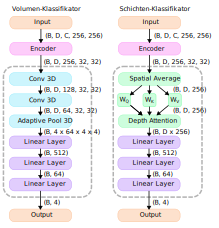
\includegraphics[width=0.9\linewidth]{Figures/Klassifikatoren.png}
  \caption{Architektur der beiden Klassifikatoren. Der Encoder wird jeweils modular ausgetauscht. 
  Links zu sehen ist die Architektur des \textit{Volumen-Klassifikators}, der die Merkmale, die der Encoder generiert, als Volumen interpretiert und mithilfe von 3D-Faltungen und Pooling daraus eine Repräsentation erzeugt.
  Diese Repräsentation wird anschließend durch Linear Layers in vier Ausgabe-Klassen umgeformt.
  Rechts ist der \textit{Schichten-Klassifikator} zu sehen.
  Die räumlichen X- und Y-Dimensionen werden im \textit{Schichten-Klassifikator} durch einen spatial average zusammengefasst.
  Durch eine Multihead Attention mit vier Attention-Köpfen und Embedding-Dimension 256 wird dann eine Repräsentation aus den individuellen Schichten der Merkmale erstellt.
  Lineare Layers formen anschließend die Repräsentation zu den vier Klassen um.}
  \label{fig:classifiers}
\end{figure}
\noindent
Der erste Klassifikator wird hier \textit{Volumen-Klassifikator} genannt.
Er interpretiert die Merkmale, die der Encoder generiert, als Volumen und generiert daraus mithilfe von 3D-Faltungen und Pooling eine neue Repräsentation.
Diese Repräsentation wird dann durch Linear Layers zu vier Ausgabe-Klassen umgeformt.
Die Idee des \textit{Volumen-Klassifikators} ist es, die Merkmale, die der Encoder generiert, möglichst vollständig zu erfassen und alle räumlichen Beziehungen, auch in Z-Richtung, festzustellen.
Hierbei ist das Ziel, dass durch die 3D-Faltungen eine domänenspezifische Interpretation der Merkmale gelernt wird, sodass die neuen Merkmale nach dem anschließenden Pooling aussagekräftig und niederdimensional sind.\\[0.5\baselineskip]
Außerdem wird hier der \textit{Schichten-Klassifikator} eingeführt.
Der \textit{Schichten-Klassifikator} betrachtet die einzelnen Schichten des Bilds anhand der individuellen Schichten, die der Encoder ausgibt, mithilfe eines Self-Attention-Mechanismus über die Z-Dimension. 
Dazu werden die räumlichen X- und Y-Dimensionen durch einen spatial average zusammengefasst.
Durch eine Multihead Attention mit vier Attention-Köpfen und Embedding-Dimension 256 wird eine Repräsentation aus den individuellen Schichten der Merkmale erstellt.
Lineare Layers formen anschließend die Repräsentation zu den vier Klassen um.
Für den \textit{Schichten-Klassifikator} ist das Ziel, dass durch die Vereinfachung der Daten aussagekräftige, schichtenweise Merkmale entstehen und dass diese räumlich invariant sind, da der betrachtete Nucleus in den Bildfenstern zentriert ist.
\newpage
\section{Segmentierung}
\subsection{Modelle}\label{sec:Seg_Modelle}
Für die Instanzsegmentierung der Nuclei werden die folgenden drei Modelle eingesetzt:
\begin{itemize}
  \item Ein Modell des nnU-Net Framework, das selbstkonfigurierte Modelle basierend auf der U-Net-Architektur erstellt \cite{isensee2021nnu}.
  \item Das DeepCell-Caliban-Modell, das Bildfaltungen und speziell entwickelten Nachverarbeitungsstrategien vereint.
  \item Cellpose-SAM, das die Architekturen der Cellpose-Modelle mit der Architektur und den Gewichten des Foundation-Model \ac{sam} vereint. 

\end{itemize}

\subsection{Nachverarbeitungsmethoden}\label{sec:Seg_PostProc}
Zur Nachbearbeitung der Instanzsegmentierungsmasken wird der Instanztrenner eingeführt.
Diese Methode dient dazu, separate Instanzen mit derselben numerischen Annotation (IDs) zu trennen und mit einzigartigen Zahlenwerten zu versehen. 
Pro Instanz werden hierzu ein zufälliges Pixel betrachtet und davon ausgehend alle Pixel mit direkter Verbindung über die Segmentierungsmaske gesucht.
Diese verbundenen Pixel werden als neue einzigartige Instanzen abgelegt, bis keine Pixel ohne Verbindung übrig bleiben. 
Eine weitere Methode der Nachbearbeitung, die auf Segmentierungsmasken eingesetzt werden kann, ist der Watershed-Algorithmus. %(siehe Abschnitt \ref{sec:Segmentierung}).
Der Algorithmus trennt überlagerte Instanzen, die das Modell als einzelne Instanzen segmentiert hat. 
%\begin{algorithm}
%\caption{Watershed-Nachbearbeitung zur Trennung überlappender Instanzen}\label{alg:watershed}
%\begin{algorithmic}
%\REQUIRE $maske_\text{instanz}$
%\ENSURE $maske_\text{refined}$
%
%\STATE $distanz \gets \text{DistanzTransformation}(maske_\text{instanz})$
%\STATE $marker \gets \text{LokaleMaxima}(distanz)$
%\STATE $gradient \gets -distance$
%\STATE $maske_\text{refined} \gets \text{Watershed}(gradient, marker)$
%
%\FOR{Region $r_i$ in $maske_\text{refined}$}
%  \IF{$Flaeche(r_i) < \tau$}
%    \IF{$r_i$ grenzt an größere Nachberregion $r_n$}
%      \STATE Vereinige $r_i$ mit $r_n$
%    \ELSE
%      \STATE Entferne $r_i$
%    \ENDIF
%  \ENDIF
%\ENDFOR
%
%\RETURN $maske_\text{refined}$
%\end{algorithmic}
%\end{algorithm}

% !TeX root = ../Thesis.tex

\chapter{Implementation} \label{ch:Implementation}
If appropriate and not done in the previous chapter, describe the implementation of your method.


\section{Überblick}
Im nachfolgenden Kapitel wird die Implementierung aller relevanten Methoden erklärt. Hierbei steht die praktische Anwendung dieser Methoden in Form von Nutzerschnittstellen oder als Entwicklerskript auf ausgewiesener Hardware im Vordergrund.

\section{Segmentierungsnetze}
\begin{itemize}
    \item Wie sind die Netze je eingebunden?
    \item Welche Hardware?
    \item Welche Vor-/Nachverarbeitung?
\end{itemize}

\section{Labeling App}
Um den Klassifikator zu trainieren werden \ac{gt} zu einigen Zieldaten mithilfe der Labeling App erstellt. 
Als Frontend dieser App dient eine dash Anwendung die eine einfache html \ac{gui} bereitstellt. 
Das Backend ist mit Python erstellt und die gesammelten Daten werden als JSON gespeichert.
Hierzu ist ein Docker mit Zugriff auf das lokale Dateiensystem versehen und über Kubernetes betrieben.
\begin{figure}
    \centering
    \includegraphics[width=0.98\linewidth]{Figures/GUI_Labeling_App.png}
    \caption{Die Grafik zeigt die \ac{gui} der Labeling App. In der Mitte wird die Zelle angezeigt, die gelabelt werden soll und links sind Bedienelemente zu sehen. Unter der dargestellten Zelle befindet sich ein Schieberegler, der die Navigation entlang der Z-Achse ermöglicht. Über die Bedienelemente kann der/die Nutzer*In zwischen Bildern und Zellen umschalten, die Klasse der Zelle bestimmen, den gezeigten Ausschnitt mit prozentualen Schwellenwerten normalisieren und und die Fenstergröße ändern.}
    \label{fig:Labeling_App}
\end{figure}
Fig. \ref{fig:Labeling_App} zeigt die \ac{gui} der Labeling App. Zentral zu sehen ist ein Fenster, das einen 2D Schnitt der ausgewählten Zelle anzeigt. Darauf ist ein roter Kasten gezeichnet, der die ausgewählte Zelle umrandet, sodass Zellen, die dicht aneinander liegen unterschieden werden können. 
Mit dem Schieberegler unter dem Fenster kann ausgewählt werden, welche er Schichten in denen die Zelle anwesend ist, gezeigt werden soll. Über dem Fenster ist der Index der aktuell dargestellten Zelle und des Bilds angegeben.
Links neben dem Fenster befinden sich Bedienelemente mit den folgenden Funktionen:
\begin{itemize}
    \item \textit{Vorheriges Bild}: Vorheriges Bild auswählen.
    \item \textit{Nächstes Bild}: Nächstes Bild auswählen.
    \item \textit{Vorherige Zelle}: Vorherige Zelle auswählen.
    \item \textit{Nächste Zelle}: Näxchste Zelle auswählen.
    \item \textit{Class X}: Bestimmte Klasse als \ac{gt} der ausgewählten Zelle definieren.
    \item \textit{Nächster undefinierter}: Nächste Zelle ohne eingetragene \ac{gt} auswählen.
    \item \textit{Speichern}: Speichert manuell die festgelegten \ac{gt}s ab. Die Labeling App speichert außerdem eigenständig periodisch.
    \item \textit{Untere \% Abschneiden}: Unteren prozentualen Schwellwert wählen, der bei der nächsten Normalisierung angewandt werden soll.
    \item \textit{Obere \% Abschneiden}: Oberen prozentualen Schwellwert wählen, der bei der nächsten Normalisierung angewandt werden soll.
    \item \textit{Normalisieren}: Normalisierung lokal auf den Ausschnitt der aktuell ausgewählten Zelle anwenden. Intensitätswerte die im beziehungsweise über dem Perzentil der eingetragenen Schwellwerten werden hierbei zusammengefasst.
    \item \textit{Zoom In}: Verkleinert den anzuzeigenden Ausschnitt.    
    \item \textit{Zoom Out}: Vergrößert den anzuzeigenden Ausschnitt.    
\end{itemize}

Für das Backend sind einige Python Skripte direkt im Docker mounted. 
Da die wichtigste Anforderung der Anwendung die nutzerfreundliche Bedienung ist, sind alle Berechnungen, die während der Nutzung der Labeling App ausgeführt werden, darauf ausgelegt die Rechnenzeit zu minimieren. 
Hierzu werden alle Bilder und Masken bei der Initialisierung der App in den cache geladen.
Des Weiteren ist eine Klasse angelegt, die separat noch das aktuell ausgewählte Bild und die ausgewählte Zelle speichert. 
Erst wenn eine Änderung der Auswahl ausgeführt wird, wird eine neue Zelle oder ein neues gesamtes Bild geladen und selbst dann lediglich aus dem cache. 


%% !TeX root = ../Thesis.tex

\chapter{Data} \label{ch:Data}
Describe the data sets you use. If you have done some experimental work, change the title to experiments (or add a chapter) and describe them.


\section{Überblick}
% !TeX root = ../Thesis.tex

\chapter{Results} \label{ch:results}
%In this chapter, the results are shown and discussed. Use an appropriate presentation of the results, e.g., tables, diagrams, plots. Be aware of statements that are too general.


\section{Überblick}

\section{Segmentierung}
Für die Wahl eines Segmentierungsnetzes wird in Kapitel \ref{ch:NewMethods} das Bewertungskriterium \ac{ipq} eingeführt.
Außerdem wird in Kapitel \ref{ch:NewMethods} der annotierte S\_BIAD1518Datensatz vorgestellt.
Die \ac{ipq} wird auf dem Datensatz mit den Masken von drei vortrainierten Segmentierungsnetzen und, zur Validierung, mit der \ac{gt} ausgeführt.
Die Masken unterscheiden sich optisch stark (siehe Abb. \ref{fig:example_masks}), was sich auch in starken Unterschieden in der \ac{ipq} äußert.
\begin{figure}[htbp]
    \centering
    \begin{subfigure}[t]{0.24\textwidth}
        \includegraphics[width=\linewidth]{Figures/Deepcell_Mask_Example.png}
        \caption{Deepcell Maske}
        \label{fig:DeepcellMaske}
    \end{subfigure}
    \hfill
    \begin{subfigure}[t]{0.24\textwidth}
        \includegraphics[width=\linewidth]{Figures/nnUNet_Mask_Example.png}
        \caption{nnUNet Maske}
        \label{fig:nnUNetMaske}
    \end{subfigure}
    \hfill
    \begin{subfigure}[t]{0.24\textwidth}
        \includegraphics[width=\linewidth]{Figures/CellposeSam_Mask_Example.png}
        \caption{CellposeSam Maske}
        \label{fig:CellposeSamMaske}
    \end{subfigure}
    \hfill
    \begin{subfigure}[t]{0.24\textwidth}
        \includegraphics[width=\linewidth]{Figures/gt_Mask_Example.png}
        \caption{\ac{gt} Maske}
        \label{fig:gtMaske}
    \end{subfigure}
    \caption{Darstellung der Segmentierungsmasken der verschiedenen Segmentierungsnetze als Konturen auf einem zweidimensionalen Durchschnitt einer Stichprobe des S\_BIAD1518 Datensatzes.}
    \label{fig:example_masks}
\end{figure}
\newline
Die Ergebnisse jedes Segmentierungsnetzes sind einzeln und für jedes Bild im Appendix \ref{supp:ipq} angehängt. 
Eine Zusammenfassung der Ergebnisse ist in den Boxplots in Abb. \ref{fig:boxplots_ipq} gegeben.
Das zentrale Ergebnis ist, dass CellposeSAM die besten \ac{ipq}-Werte erzielt. 
Mit einem Mittelwert von \num{0.64} ist die \ac{ipq} von CellposeSAM signifikant höher als der Mittelwert bei nnUNet (\num{0.04}) und Deepcell (\num{0.02}), mit entsprechenden p-Werten von \num{1.80e-80} bzw. \num{1.59e-81} bei einseitigen T-Tests. 
Dennoch zeigt sich, dass CellposeSAM lediglich in der Kategorie Segmentatierungs-Qualität (SQ) sowohl den höchsten Median als auch den höchsten Mittelwert erreicht. 
Die Recognition-Qualität (RQ) der nnUNet-Masken ist signifikant höher als die der CellposeSAM-Masken (p-Wert: \num{3.4764e-06}), und ebenso die Injektive Qualität (IQ) der Deepcell-Masken (p-Wert: \num{6.7763e-08}).
Obwohl nnUNet und Deepcell jeweils eine Metrik dominieren, wird ihr \ac{ipq}-Wert durch die beiden schlechten Faktoren stark heruntergezogen, während CellposeSAM in jeder Metrik gut, wenn auch nicht am besten, abschneidet.
Außerdem zeigen die Boxplots viele Ausreißer in den Daten, was den Unterschieden der Bildkategorien, die der Datensatz enthält, geschuldet sein könnte.

\begin{figure}[t]
    \centering
    \includegraphics[width=\linewidth]{Figures/Segmentation_Boxplots}
    \caption{Boxplots der Ergebnisse der \ac{ipq} Berechnungen mit Faktoren \textit{$k_1$}, \textit{$k_2$} und \textit{$k_3$} jeweils gleich eins. 
    Die X-Achse unterteilt die Daten in die Kriterien Segmentatierungs-Qualität (SQ), Recognition Qualität (RQ), Injektivitäts-Qualität (IQ) und \acf{ipq}, wie in der Formel \ref{eq:ipq} beschrieben. 
    Für jede Metrik sind drei farbige Boxplots zu sehen, einer für jedes Segmentierungsnetz.
    Die Boxplots visualisieren hierbei die Verteilung der Metriken.
    Die Box repräsentiert das Interquartilsintervall (25.–75. Perzentil), wobei der Median als Linie innerhalb der Box dargestellt ist. 
    Die sogenannten Whisker reichen bis zum 1,5-fachen des Interquartilsabstands über die Box hinaus. 
    Darüber hinausgehende Punkte gelten als Ausreißer und werden einzeln dargestellt.}
    \label{fig:boxplots_ipq}
\end{figure}


\section{Klassifikation}
Die in Kapitel \ref{ch:NewMethods} vorgestellten Methoden zur Klassifikation werden anhand eines separaten Anteils des manuell gelabelten Datensatzes getestet.
Die Genauigkeit, also der prozentuale Anteil richtiger Vorhersagen, auf dem Test-Anteil des Zieldatensatzes wird als Kriterium verwendet.
Da die Modelle während des Trainings rauschbehaftete Verläufe der Genauigkeit und es zu Overfitting kommen kann, wird nicht das Modell am Ende des Trainings zur Evaluation eingesetzt, sondern das Modell der Trainingsepoche, in der die Genauigkeit am höchsten ist.
\textit{TODO: Trainings-Verlauf Kurve einfügen}
\textit{TODO: Text zu den Abbildungen, t-Tests ausführen}
In Abb. \ref{fig:bars_encoders} ist die Genauigkeit der Klassifikatoren pro Encoder gegeben.

\begin{figure}
    \centering\includegraphics[width=\linewidth]{Figures/encoders_compare.png}
    \caption{Das Balkendiagramm zeigt an der Y-Achse die Genauigkeit der Klassifikatoren unter Verwendung der verschiedenen Encoder.
    Auf der X-Achse sind die Encoder als Gruppen aufgetragen.
    Jede Gruppe enthält einen Maximalwert (Orange) und einen Durchschnittswert (Blau), da jeder Encoder mit verschiedenen Kombinationen von Methoden getestet wird.
    Die Encoder sind nach aufsteigendem Maximalwert von links nach rechts sortiert.
    }
    \label{fig:bars_encoders}
\end{figure}
\begin{figure}
    \centering\includegraphics[width=\linewidth]{Figures/encodersVdecoder.png}
    \caption{Das Balkendiagramm zeigt den Genauigkeitswert der Klassifikatoren unter Verwendung eines bestimmten Decoder.
    Auf der Y-Achse ist der Durchschnitt der Genauigkeiten der besten Trainingsepoche aller Klassifikatoren, die diesen Decoder nutzen, aufgetragen. 
    Die X-Achse zeigt Gruppen von Encodern, jeweils besetzt mit einem Wert für den Schichten- und den Volumen-Klassifikator.
    Rechts zu sehen sind Balken, die den Durchschnitt der Werte aller Encoder, abhängig von dem Decoder, zeigen.}
    \label{fig:bars_decoders}
\end{figure}
\begin{figure}
    \centering\includegraphics[width=\linewidth]{Figures/encodersVchannel1.png}
    \caption{Das Balkendiagramm zeigt den Genauigkeitswert der Klassifikatoren unter Verwendung einer bestimmten Vorverarbeitungsart.
    Auf der Y-Achse ist der Durchschnitt der Genauigkeiten der besten Trainingsepoche aller Klassifikatoren, die diese Vorverarbeitungsart nutzen, aufgetragen. 
    Die X-Achse zeigt Gruppen von Encodern, jeweils besetzt mit einem Wert für den Typ Eins, der den Nucleus-Kanal des Bilds mit der Segmentierungsmaske ersetzt, und Typ 2, der eine Distanztransformation auf den Nucleus-Kanal anwendet.
    Rechts zu sehen sind Balken, die den Durchschnitt der Werte aller Encoder, abhängig von der Vorverarbeitungsmethode, zeigen.}
    \label{fig:bars_channel1}
\end{figure}
\begin{figure}
    \centering\includegraphics[width=\linewidth]{Figures/encodersVpretrain.png}
    \caption{Die Heatmap zeigt die Genauigkeiten der Klassifikatoren unter Verwendung der verschiedenen Vortrainingsmethoden.
    Auf der Y-Achse sind die verschiedenen Encoder aufgetragen.
    Die X-Achse stellt die getesteten Methoden des Vortrainings dar.
    Die Farbe der Felder und der Wert darin zeigen die Durchschnitte der Genauigkeiten aller Klassifikatoren, die die entsprechende Vortrainingsmethode nutzen.
    Die letzte Zeile zeigt den Durchschnitt der Werte aller Encoder, abhängig von der Vortrainingsmethode.}
    \label{fig:heatmap_pretrain}
\end{figure}
% !TeX root = ../Thesis.tex

\chapter{Diskussion}\label{ch:Discussion}
%Repeat the problem and its relevance, as well as the contribution (plus quantitative results). Look back at what you have written in the introduction. 

\section{Überblick}
Die nachfolgenden Kapitel diskutieren die Ergebnisse der vorliegenden Arbeit.
Dabei wird sowohl auf die quantitative Auswertung der durchgeführten Experimente eingegangen, als auch auf die Bewertung der angewandten Methoden.
Es wird gezeigt, dass die neu entwickelte \ac{ipq}-Metrik geeignet ist um Instanzsegmentierungsmodelle, im Bezug auf ihre Eignung interpretierbare Merkmale zu extrahieren, zu bewerten.

\section{Segmentierung}
Durch einen Vergleich der Masken mit der Annotationen in Abb. \ref{fig:boxplots_ipq} und ihren zugehörigen Ergebnissen der einzelnen Bewertungskriterien sind die Schwächen und Stärken der individuellen Netze ersichtlich.
Die nnUNet-Masken sind sichtbar kleiner als die Nucleus-Instanzen, was eine schlechte Segmentierungsqualität bedingt.
Oft zerteilen mehrere nnuNet-Masken eine Nucleus-Instanz, was von der Injektiven Qualität bestraft wird.
Wie auch die gute Recognition Qualität zeigt, findet dafür nnUNet sehr zuverlässig die anwesenden Nuclei mit mindestens einer Maske.
Mit dem nnUNet-Modell sind außerdem aufgrund der kleinen Segmente, die das Modell vorhersagt, Überschneidungen zwischen Annotationsmaske und Segmentierungsmaske gering. 
Ein Weg die Leistung des Modells im Bezug auf die \ac{ipq}-Metrik zu verbessern ist deshalb vermutlich das Modell, beispielsweise durch fine-tuning, auf größere Segmente anzupassen.
Eingangsdaten, beispielsweise durch einen Mittelwert-Filter, kleiner zu dimensionieren und mehrere Bilder aneinandergereiht einzugeben kann auch zu Verbesserungen führen, dabei besteht allerdings das Risiko, dass der Informationsverlust durch den Filter das Ergebnis negativ beeinflusst. \newline
Deepcell (siehe Abb. \ref{fig:DeepcellMaske}) übersegmentiert die Nuclei, wodurch die Segmentierungsqualität stark abnimmt.
Das Ergebnis sind Masken, die intuitiv zu groß sind und oft mehr als einen Nucleus enthalten.
Das bedeutet auch, dass einige Nuclei nicht von einer eigenen Maske gefunden werden, was sie als \ac{fn}-Instanzen kategorisiert und eine schlechte Recognition Qualität bedingt.
Durch diese Übersegmentierung wird vermieden, dass Instanzen der Annotation durch die Deepcell-Masken geteilt werden, was zu einer guten Injektiven Qualität führt.
Außerdem ist durch die großen Segmente die Segmentierungs-Qualität besonders schlecht, weil die Größe der Segmente den Nenner der \ac{iou} erhöht.
Die Deepcell-Masken können im Bezug auf die \ac{ipq} von weiterer Nachverarbeitung profitieren.
Mithilfe eines Erosion-Filter können die Masken kleiner gemacht werden, was auch zu einer besseren Leistung der Watershed-Nachverarbeitung führen kann.
Umgekehrt kann nach der Erosion die Maske aber auch Kerben an der Kontur einzelner Instanzen aufweisen, die zur Spaltung der Instanz durch die Watershed-Nachverarbeitung führen.
Auch für das Deepcell-Modell ist fine-tuning zu Anpassung an die Größe der Nuclei vermutlich ein Weg die Qualität zu verbessern.\newline
Sowohl für das nnUNet-, als auch für das Deepcell-Modell gibt es zwar Vorschläge für Methoden zur Verbesserung der \ac{ipq} auf dem Benchmark-Datensatz, aber der Übertrag der Effektivität dieser Methoden auf die Zieldaten ist fraglich.
Die Bilddomäne und auch die Eigenschaften wie Größe, Exzentrizität und Rundheit der Zieldaten unterscheiden sich von denen des Benchmark.
Da keine Annotationen für die Instanzsegmentierung der Zieldaten verfügbar sind wird von der Anwenden der Methoden im Zuge dieser Arbeit abgesehen, um kein Overfitting auf den Benchmark-Datensatz zu riskieren. \newline


\begin{figure}[h]
    \centering
    \begin{subfigure}[t]{0.24\textwidth}
        \includegraphics[width=\linewidth]{Figures/ideal_gt.pdf}
        \caption{Annotationsmaske als Kontur.}
        \label{fig:ideal_gt}
    \end{subfigure}
    \hfill
    \begin{subfigure}[t]{0.24\textwidth}
        \includegraphics[width=\linewidth]{Figures/ideal_IQ.pdf}
        \caption{Idealer IQ-Fehler. Ein optimal segmentierter Nucleus wird in zwei Segmente gespalten.}
        \label{fig:ideal_IQ}
    \end{subfigure}
    \hfill
    \begin{subfigure}[t]{0.24\textwidth}
        \includegraphics[width=\linewidth]{Figures/ideal_RQ.pdf}
        \caption{Idealer RQ-Fehler. Es werden zusätzliche Nuclei halluziniert.}
        \label{fig:ideal_RQ}
    \end{subfigure}
    \hfill
    \begin{subfigure}[t]{0.24\textwidth}
        \includegraphics[width=\linewidth]{Figures/ideal_SQ.pdf}
        \caption{Idealer SQ-Fehler. Der Nucleus wird in doppelter Größe vorhergesagt.}
        \label{fig:ideal_SQ}
    \end{subfigure}
    \caption{Darstellung der Segmentierungsmasken verschiedener idealer Fehler und der Annotation als Kontur.}
    \label{fig:ideal_example_masks}
\end{figure}
Anhand der Interpretation der Werte und der exemplarischen Fehler in Abb. \ref{fig:ipq_examples} wird die Effektivität der neu entwickelten \ac{ipq}-Metrik ersichtlich.
Verschiedene Fehlerarten, die zu unterschiedlichen Verfälschungen der interpretierbaren Merkmale der Daten führen werden gezielt von der Metrik erfasst.
In der Praxis gehen die Fehler oft mit Fehlern einer anderen Art einher, was daran liegt, dass die Modelle nicht dem selben Denkverhalten folgen wie ein menschlicher Betrachter.
Abb. \ref{fig:ideal_example_masks} zeigt idealisiert die Fehlerarten, die mit der \ac{ipq}-Metrik erkannt werden.
Alle Fehler führen für den betrachteten Nucleus zu einem Faktor von 0,5 in ihrer Kategorie und einem optimalen Wert von 1 in den anderen Kategorien.
Hier wird deutlich, dass die Metrik geeignet ist um: 
\begin{itemize}
    \item Fehleinschätzungen der Konzentration von Nuclei durch den neu eingeführten IQ-Wert zu bestrafen,
    \item Fehleinschätzungen des Volumens der Nuclei durch einen geringen SQ-Wert zu bestrafen und
    \item Fehleinschätzungen der Anzahl der Nuclei durch einen geringen RQ-Wert zu bestrafen.
\end{itemize}
\section{Klassifikation}
Die Interpretation der Ergebnisse der Genauigkeit von Klassifikatoren mit verschiedenen Encodern, Decodern, Vorverarbeitungsmethoden und Vortrainingsmethoden legt einige Aussagen über Effektivität der Methoden nahe.
Vor allem aber zeigen die Ergebnisse, dass die Anwendung der optimalen Klassifikator-Methoden einen sehr hoch signifikanten Einfluss auf die Genauigkeit des Klassifikators hat.
Die 3D-Zelldaten-Pipeline findet diese optimalen Methoden effizient.
Wie die Ergebnisse zeigen, ermöglicht die Anwendung der 3D-Zelldaten-Pipeline das Training eines Klassifikators, der deutlich leistungsfähiger ist als ein Klassifikator mit zufällig gewählten Methoden – und das ganz ohne Programmierkenntnisse oder Vorerfahrung mit Deep-Learning-Methoden seitens der Anwender*innen\newline
%Encoder
...
\newline 
%Decodern
Der Volumen-Klassifikator ist signifikant besser als der Schichten-Klassifikator (siehe Kapitel \ref{sec:resultsClassifier}).
Dieses Erkenntnis legt nahe, dass die dreidimensionalen Faltungsschichten besser den zusammenhang der Merkmale erfassen können, als der Attention-Mechanismus des Schichten-Klassifikators.
Das kann daran liegen, dass die dreidimensionale Faltung räumliche Mittlungen nur mit gelernten Gewichten durchführt, während die Spatial Average Operation großflächig die räumliche Beziehung der Merkmale vernachlässigt.
Außerdem ist es möglich, dass die für die Klassifikation ausschlaggebenden Informationen nicht ausreichend entlang der Z-Dimension erhalten sind, was zu einer schlechten Leistung des tiefen fokusierten Schichten-Klassifikators führt. 
Stattdessen können auch die Kombination räumlicher Merkmale und der Merkmale entlang der Z-Achse wichtig sein, was die gute Leistung des Volumen-Klassifikators bedingen kann.
Da der Schichten-Klassifikator mit dem ConvNeXt Encoder im Durchschnitt höhere Genauigkeiten erzielt, als mit dem Volumen-Klassifikator, ist die Abwägung zwischen den beiden Methoden dennoch für zukünftige Anwendungen sinnvoll. 
Bestimmte Encoder erfassen die relevanten Merkmale auf unterschiedliche Weise und beide Decoder haben das Potential mit bestimmten Merkmalsräumen besonders gut zu synergieren. 
Besonders da die ImageNet-Encoder nicht auf dreidimensionale Eingabedaten vortrainiert werden ist die Abwägung zwischen einem Fokus auf die Merkmale entlang der Z-Achse und räumlichen Merkmalen essenziell.
Auch für zukünftige Encoder besteht die Möglichkeit, dass sie Beziehungen von Merkmalen innerhalb einer 2D-Schicht der Eingabedaten so effizient und einheitlich zusammenfassen, dass der Attention-Mechanismus des Schichten-Klassifikators die Informationen besser als der Volumen-Klassifikator erhalten kann. 
\newline 
%Vorverarbeitungsmethoden
Auch für Vorverarbeitung ist eine signifikant bessere Methode zu erkennen. 
Die Masken-Methode ist signifikant besser als die Distanz-Methode.
Kapitel \ref{sec:MethodsClassifier} beschreibt den Vorteil und das Risiko der Methoden.
Insbesondere der Vorteil der Masken-Methode wird an den Ergebnissen sichtbar. 
Anhand der GradCAM-Heatmap in Abb. \ref{fig:gradCAM} wird abgeleitet, dass die Oberflächenmerkmale der Nuclei für die Klassifikation keine Rolle spielen.
Ein Risiko der Masken-Methode ist ein Qualitäts-Verlust aufgrund der Eliminierung der Oberflächenmerkmale, aber selbst mit der Distanz-Methode werden diese Merkmale nicht betrachtet.
Die Masken-Methode hebt die Geometrie der Nuclei besonders hervor und sowohl die statistische Betrachtung der Ergebnisse als auch die GradCAM-Heatmaps legen nahe, dass diese Geometrie besonders wichtig für die Klassifikation der Nuclei ist.
Mit der Distanz-Methode wird nicht nur die Geometrie nicht besonders hervorgehoben, unter Umständen wird sie sogar durch direkt umliegende Nuclei beeinträchtigt.
Da die Segmentierungs-Maske außer in der Distanztransformation nicht in den Daten der Distanz-Methode vorhanden ist, geht die Information über die Kanten vollständig verloren, überall umliegende Nuclei den betrachteten Nucleus direkt berühren.
Der berührende Nucleus wird in diesem Fall als Teil des betrachteten Objekts interpretiert.
Für kommende Anwendungen ist dennoch die Überlegung der Auswahl einer Vorverarbeitungsmethode interessant, da die Nuclei von anderen Zieldaten Informationen auf der Oberfläche tragen können, die für die Klassifikation wichtig sind.\newline 
%Vortrainingsmethoden
Der Einfluss der Vortrainingsmethoden ist besonders bedeutsam.
Mit dem fully-supervised Vortraining ist die durchschnittliche Genauigkeit höher und auch konsistenter als mit anderen Vortrainingsmethoden.
Das legt nahe, dass das rechenaufwändige Vortraining auf dem ImageNet-Datensatz mit den diversen Klassen und zahlreichen Stichproben für jede Klasse einen stark generalisierten Merkmalsraum erzeugt.
Obwohl die Bilddomäne biologischer Zelldaten stark von den Bildern des ImageNet-Datensatz abweicht werden bedeutsame Bildmerkmale extrahiert.
Auch bei der Adaption von 2D-Encodern zu 3D-Encodern bleibt der Merkmalsraum der fully-supervised-vortrainierten Encoder sinnvoll.
Da die Zieldaten niemals vom Encoder gesehen werden ist Overfitting weitgehend ausgeschlossen, was die geringe Varianz der Genauigkeiten innerhalb der fully-supervised-vortrainierten Klassifikatoren erklärt.\newline
Auch komplett ohne Vortrainig wird ein sinnvoller Merkmalsraum gelernt und die Klassifikatoren erreichen teilweise hohe Genauigkeitswerte. 
Der Swin V2-Encoider hat ohne Vortraining nur 50\% Genauigkeit erreicht, was vermutlich daran liegt, dass die aufwändige Transformer-Architektur nicht ausreichen mit dem geringen Trainingsumfang der Zieldaten lernen kann.
Es wird keine sinnvolle Merkmalsextraktion gelernt, bevor der Encoder mit dem Overfitting beginnt.
Das legt auch nahe, dass Encoder mit besonders hoher Parameteranzahl nicht ohne ImageNet-Vortraining auskommen.
Die Beobachtung, dass der kleinste Encoder, der ResNet18-Encoder, ohne Vortraining das beste Ergebnis geliefert hat unterstützt diese Aussage noch.
Mit dem ResNet18-Encoder ist es möglich das ImageNet-Vortaining auszulassen und die Merkmalsextraktion direkt durch die Zieldaten zu lernen. 
Insgesamt ergibt sich hierdurch eine geringere Generalisierbarkeit, aber für den angewandten Datensatz wird dafür die Genauigkeit besser.
Die verbleibenden Encoder sind etwas weniger genau, wenn das ImageNet-Vortraining ausgelassen wird. 
Das liegt vermutlich daran, dass diese relativ großen Encoder zum einen aus den wenigen Stützvektoren der Repräsentation der Eingangsdaten keinen ausreichenden Merkmalsraum aufspannen können und zum anderen daran, dass der Klassifikator-Kopf daraufhin die Beziehung zwischen Merkmalen und Entscheidung nur schwach generalisiert lernen kann. 
Dennoch ist die Genauigkeit auch ohne Vortaining annehmbar, vor allem da mithilfe der 3D-Zelldaten-Pipeline auch ein optimaler Encoder, wie hier der ResNet18-Encoder passed zur Vortrainingsmethode gewählt wird.
Die durchschnittlich geringere Genauigkeit ist deshalb nicht wichtig, da das Optimum besser ist. \newline
Allerdings ist der Merkmalsraum ohne Vortraining und auch nach dem fully-supervised-Vortraining nicht geeignet um besonders Myotuben-Kerne und Schwannzellen-Kerne zu unterscheiden. 
Die Unterscheidung dieser Klassen ist für die vorliegenden Daten wichtiger, als die Unterscheidung der "Andere"-Klasse und der Debris-Klasse.
In Abb. \ref{fig:scatter} sind zwei exemplarische Merkmalsräume als 2D-Projektion zu sehen.
\begin{figure}[H]
    \centering
    \includegraphics[width=0.9\linewidth]{Figures/scatter.pdf}    
    \caption{Die Scatterplots zeigen 2D-Projektionen des Merkmalraums von zwei Klassifikatoren durch TSNE.
    Der linke Scatterplot zeigt den Merkmalsraum eines ImageNet-vortrainierten Klassifikatiors, der rechte eines semi-supervised-vortrainierten Klassifikators.
    Die Werte der X- und Y-Achse sind arbiträre Aktivierungsintensitäten ohne physische Interpretation. 
    }
    \label{fig:scatter}
\end{figure}
Durch die Projektion gehen Distanzen zwischen den Stichproben entlang der vielen Dimensionen des Merkmalvektors verloren, aber mithilfe der TSNE ist die Abbildung als Übersicht dennoch geeignet.
Der linke Merkmalsraum ist aus einem ImageNet-Vortraining entstanden, der rechte durch ein semi-supervised-Vortraining.
Zu sehen ist, dass im linken Scatterplot die Klassen Eins und Vier, also Myotuben- und Schwannzellen-Nuclei eine besonders starke Überschneidung haben. 
Für die Klassen Zwei und Drei sind dagegen seperate Cluster erkennbar.
Im rechten Scatterplot ist das Schwannzellen-Klassen-Cluster zwar immernoch nicht weit entfernt von anderen Clustern, aber wesentlich kompakter, als in der linken Abbildung.\newline
Für die Unterscheidung der Myotuben- und Schwannzellen-Nuclei ist also das Vortraining mit semi-supervised-Annotationen besonders hilfreich. 
Vermutlich wird durch das Exzessive Vortraining auf den Zieldaten dem Encoder ein so gut generalisierter Merkmalsraum antrainiert, dass der Decoder die beiden Klassen trotz der Überschneidungen ihrer Merkmale trennen kann.
In den Zieldaten hingegen sind diese Merkmale häufig vertreten und werden deshalb so hochauflösend extrahiert, dass es zur Trennung der Klassen reicht.Die Auflösung genau der Merkmale die für das Trennen der beiden Klassen nötig sind, ist nach dem ImageNet-Datensatz-Vortraining vermutlich nicht sehr hoch.\newline
Die durchschnittliche Genauigkeit der semi-supervised-vortrainierten Klassifikatoren ist zwar geringer, als die der anderen Vortrainingsmethoden, dafür ist der entstandene Klassifikator aber besser generalisiert.
Da im Test-Anteil der annotierten Daten nur acht der 81 Stichproben die Klsse Schwannzellen-Nucleus besitzen ist die Genauigkeit der semi-supervised-vortrainierten Klassifikatoren nicht zwingend repräsentativ für die tatsächliche Leistung.
Für die Wahl einer Vortrainingsmethode müssen demnach die genauen Ziele der Anwendung feststehen.
Wenn einzelne Klassen besonders wichtig für die Interpretation der Ergebnisse sind, aber nicht häufig vorkommen lohnt es sich den semi-supervised-Ansatz zu testen, um eventuell durch die hohe Generalisierungsfähigkeit einen besseren Klassifikator zu erhalten.\newline 

% !TeX root = ../Thesis.tex

\chapter{Zusammenfassung und Ausblick}\label{ch:Conclusion}

Die vorliegende Arbeit befasst sich mit der automatisierten Optimierung von Deep-Learing-Methoden.
In der theoretischen Grundlage sind etablierte Deep-Learing-Methoden für die Instanzsegmentierung und Klassifikation gegeben.
Vor allem Methoden die für biologische 3D-Daten geeignet sind werden beleuchtet.
Zusätzlich sind Methoden zusammengefasst, die für die Anwendung, Auswertung und Visualisierung der vorgestellten Methoden wichtig sind.
Zu den Methoden aus der Literatur wird außerdem eine Literaturrecherche angestellt, die explizit aktuelle Forschung in dem Bereich darstellt.
Hiernach wird dargestellt, was bisher die Lücken in der Literatur sind.
Für dreidimensionale Bilddaten sind zwar sowol Methoden zur Segmentierung als auch zur Klassifikation verfügbar, aber kein umfassendes Framework, dass die Anwendung, den Vergleich und die Optimierung automatisiert.
Dementsprechend wird das Ziel der vorliegenden Arbeit definiert.
Durch die Arbeit soll der Aufwand ständig wiederkehrender Überlegungen und Vergleiche eliminiert werden, indem die Methodenauswahl und Evaluation von Deep-Learning-Methoden zur panoptischen Segmentierung von biologischen 3D-Daten automatisiert wird.\\[0.5\baselineskip]
In der Methodik der Arbeit werden hierzu einige neu entwickelte Methoden eingeführt.
Die \acf{ipq} ist eine Metrik zur Bewertung von Instanzsegmentierungsmodellen in Bezug auf ihre Eignung interpretierbare Eigenschaften zu extrahieren.
Durch die Ergebnisse der durchgeführten Experimente wird deutlich, dass die \ac{ipq} effizient die Leistung von Modellen erfasst und interpretierbare Ergebnisse bietet.
Des Weiteren werden verschiedene Encoder, Klassifikations-Köpfe, Vorverarbeitungsmethoden und Vortrainingsmethoden eingeführt.
Diese Methoden sind in der 3D-Zelldaten-Pipeline implementiert, einer automatisierten Anwendung zum Vergleich der Leistungen der Methoden.
Die Anwendung umfasst außerdem die neu eingeführte Labeling-App, eine Methode zur zeiteffizienten Annotation von dreimensionalen Bild-Datensätzen. 
Mithilfe der 3D-Zelldaten-Pipeline werden Experimente an einem Datensatz von dreidimensionalen Myotuben-Zellkultur-Aufnahmen durchgeführt.
Die Ergebnisse dieser Experimente belegen die Effizienz der 3D-Zelldaten-Pipeline.
Außerdem zeigen sie, dass die Anwendung der semi-supervised-Vortrainingsmethode mit dem neu eingeführten Pseudo-Labler zwar zu einer geringeren Durchschnittsgenauigkeit, aber auch zu einer stärkeren Generalisierung des Klassifikators führt.\\[0.5\baselineskip]
In den Ergebnissen sind des Weiteren grundlegende Erkenntnisse zu den Nuclei von \linebreak Myotuben-Zellkulturen ersichtlich.
Oberflächenmerkmale von Nuclei sind nicht hilfreich für die Unterscheidung von Nucleus-Klassen.
Nur anhand ihrer Geometrie wird eine konsistente Klassenentscheidung gelernt.
Außerdem sind die Marker-Kanäle für die Klassenentscheidung genauso wichtig wie der Nucleus-Kanal.\\[0.5\baselineskip]
%Ausblick
Die Ergebnisse haben gezeigt, dass die Geometrie der Nuclei für die Klassifikation essenziell ist.
Dementsprechend ist ein mögliches Anliegen kommender Forschung die Erweiterung der \ac{ipq}-Metrik, um Veränderungen der Geometrie durch das Segmentierungsmodell explizit zu bestrafen.
Für diese Erweiterung kann ein neuer Faktor eingeführt werden, der die geometrischen Eigenschaften der Annotationen und der segmentierten Instanzen erfasst, beispielsweise als Parameter der Fourier-Entwicklung ihrer Konturen, und mit einem geeigneten Ähnlichkeitsmaß vergleicht.
In Anbetracht der Ergebnisse der Klassifikator-Methoden kann zukünftige Forschung weitere, kleinere \ac{cnn}-Encoder in Betracht ziehen, um die Hypothese zu prüfen, dass die Encoder zu groß sind um eine sinnvolle Repäsentation der räumlich relativ kleinen Nuclei zu finden. 
Mit neuen Datensätzen kann außerdem die Hypothese geprüft werden, dass die Oberflächenmerkmale von Nuclei für die Klassifikation unwichtig und die Geometrie ausschlaggebend sind, indem die neu eingeführten Vorverarbeitungsmethoden weiter verglichen werden. 
Besonders interessant ist für kommende Forschung eine fortgeführte Analyse der vorgestellten Vortrainingsmethoden.
Das semi-supervised-Vortraining führt zu einer geringeren Durchschnittsgenauigkeit, aber zu einer stärkeren Generalisierungsfähigkeit des Klassifikators.
Kommende Forschung kann die Methode weiter Optimieren, um die Durchschnittsgenauigkeit möglicherweise zu erhöhen und die Vorteile der Methode so besser anwendbar zu machen.
Hierzu können weitere Eigenschaften der Nuclei erfasst und dem Merkmalsvektor hinzugefügt werden, auf den der Label-Spreading-Algorithmus angewandt wird oder die PCA durch einen anderen Algorithmus ersetzt werden.
Außerdem kann die anschließende Trainingsroutine mit mehr Epochen und einer geringeren Lernrate durchgeführt werden.\\[0.5\baselineskip]
In Ausblick auf eine vollständige Instanzsegmentierung von Myotuben kann die panoptische Segmentierungsmaske der Nuclei genutzt werden, um Hinweise für ein Segmentierungsmodell wie \ac{sam} zu generieren.
Die Myotuben-Zellkerne liegen in den Myotuben und sind mit ihrer langen Achse entlang der Ausrichtung der Nuclei orientiert.
Anhand der Ausrichtungen und relativen Positionen der vorhergesagten Myotuben-Zellkerne können Linien gefunden werden.
Diese Linien können dem Segmentierungsmodell als Hinweise übergeben und so eventuell die Instanzsegmentierung von Myotuben ermöglicht werden.


\begin{acronym}

\acro{ki}[KI]{Künstliche Intelligenz}
\acro{gan}[GAN]{Generative Adversarial Network}
\acro{gui}[GUI]{Graphical User Interface}
\acro{sam}[SAM]{Segment Anything Model}
\acro{tsne}[t-SNE]{t-Distributed Stochastic Neighbor Embedding}
\acro{iou}[IoU]{Intersection over Union}
\acro{pq}[PQ]{Panoptic Quality}
\acro{ipq}[IPQ]{Injektive Panoptische Qualität}
\acro{tp}[TP]{True Positive}
\acro{fp}[FP]{False Positive}
%\acro{tn}[TN]{True Negative}
\acro{fn}[FN]{False Negative}
\acro{cnn}[CNN]{Convolutional Neural Network}
\acro{vit}[ViT]{Vision Transformer}


\end{acronym}

%% !TeX root = ../Thesis.tex

\chapter{Getting Started with \LaTeX} \label{ch:LatexTips}
\LaTeX\ is a typesetting system widely used in academia. It is free software and outperforms WYSIWYG  (what you see is what you get) programs like word in many ways. pdfLaTeX is commonly used to get a PDF as output. However, the development of pdfLaTeX is nearly finished. LuaLaTeX is a  successor to pdfLaTeX and also enables the use of Lua. 

In this chapter, some advice for writing a thesis with \LaTeX\ is given. The choice to use LuaLaTeX and the TeX Live distribution with the TeXworks editor is based on my personal preferences and experiences\footnote{Tim Scherr, Automated Image and Data Analysis (AIDA), \href{mailto:tim.scherr@kit.edu}{tim.scherr@kit.edu}}. Big advantages of LuaLaTeX are new packages and the Unicode support. Using a modern keyboard layout, e.g., \href{https://neo-layout.org/}{Neo}, and Unicode supporting fonts (in this document: Linux Libertine, Linux Biolinum and XITS math) allows to write more readable \LaTeX\ code. If you have some remarks, please send me an e-mail.

\section{Installation}
The installation of the TeX Live distribution on a windows system is briefly described on the \href{https://www.tug.org/texlive/acquire-netinstall.html}{\TeX\ Users Group web site}. Install biber to process bibliographies (no \href{https://texwelt.de/wissen/fragen/1909/wie-verwende-ich-biber-in-meinem-editor}{installation} needed since TeX Live 2018). BibTeX is obsolete and not recommended anymore.

For the Debian based Linux distributions Linux Mint and Ubuntu, the package manager can be used to install TeX Live. However, the provided TeX Live version may be quite old. See \href{https://wiki.ubuntuusers.de/TeX_Live/}{here}, how to get a newer version. Using the Arch Linux based Manjaro distribution enables to get an up-to-date TeX Live and biber within the package manager.

\section{Manuals}
Overleaf provides an \href{https://de.overleaf.com/learn/latex/Free_online_introduction_to_LaTeX_(part_1)}{introduction into \LaTeX} and some further information about \href{https://www.overleaf.com/learn/latex/Articles/An_Introduction_to_LuaTeX_(Part_1):_What_is_it\%E2\%80\%94and_what_makes_it_so_different\%3F}{LuaTex}. The so-called TeXdocs provide the documentation of packages such as graphicx to include graphics into the document. To open an TeXdoc, open a command-line or terminal and execute \verb|texdoc packagename| (or use google to find it). TeXdocs can be very detailed. 

\section{Document Classes}
I recommend to use the KOMA-Skript document classes scrbook (for books), scrreprt (ideal for theses), scrartcl (for articles), and scrlttr2 (for letters). This thesis template is based on the scrreprt class. The TeXdoc scrguide is a very interesting documentation, going far beyond the simple use of the KOMA-Skript classes. I really recommend to read at least the beginning of this TeXdoc. If something cannot be changed within the KOMA-Skript, it should not be changed probably.

\section{Document Structure}\label{sec:Structure}
Structure your document using chapters (\verb|\chapter{}|), sections (\verb|\section{}|), subsections (\verb|\subsection{}|), subsubsections (\verb|\subsubsection{}|), and paragraphs (\verb|\paragraph{}| or an empty line in the code). The commands \verb|\chapter*{}|, \verb|\section*{}|, … suppress the numbering and the table of contents entry.  \verb|\addchapter{}| adds an unnumbered chapter with table of contents entry.

\subsubsection{Exemplary Subsubsection}
This is an example for a subsection. Subsubsections are not numbered in this template.

\paragraph{Paragraph} This is an example for the paragraph command. In contrast to a subsubsection, no new line is started. The \verb|\paragraph{}| command sets its argument bold.

In contrast, an empty line in the code starts new indented paragraphs such as this paragraph. Paragraphs may help to improve the readability of your thesis. Be aware of \href{https://en.wikipedia.org/wiki/Widows_and_orphans}{widows and orphans}!

 Use the \verb|\label{}| and  the \verb|\ref{}| or \verb|\autoref{}| command to reference to figures, chapters, sections, tables, …, e.g., section \ref{sec:Structure}, \autoref{ch:results}, or \autoref{eq:pythagoras}. The autoref names can be changed in the header.tex file.

\section*{Exemplary Section Without Numbering}
There is no table of contents entry for this unnumbered section.

\section{Tips}
If you need some help with a package, read its texdoc first. If you do not know the command for some symbol or what package it provides, use \href{http://detexify.kirelabs.org/classify.html}{Detexify}. Detexify is a really useful tool.

Use the right click and “go to pdf“ or “go source code” to switch between your source code and pdf. The use of \verb|% !TeX root = ../Thesis.tex| in the first line of a sub-file allows to build your document without opening the main file Thesis.tex.

\subsection{Spell Checker}
Install some spell checker for your editor. For TeXworks, go to Help → A short manual for TeXworks → spell-checking.

\subsection{Settings}
Activate the line numbers in the TeXworks settings and disable the closing of the console output (Edit → Preferences → Typesetting). Set LuaLaTeX as default. Fill in your name and topic in the hypersetup in the header.tex file. If you want to write your thesis in German, set the main language to ngerman for the babel package and the documentclass in header.tex. Replace 0\_Titlepage with 0\_Titlepage\_german in the Thesis.tex file. Change the siunitx language as well. If you know your needed binding offset for the printed version, change the first optional \verb|\areaset[1.3cm]{15.3cm}{23.5cm}| argument.

\section{Math}
Use punctuation marks if you are writing some equations and embed them into your text. Describe all used variables. Useful environments are \verb|equation|, e.g., 
\begin{equation}\label{eq:pythagoras}
	a² = b² + c² \; ,
\end{equation}
\verb|align| for multiple equations with alignment, e.g., 
\begin{align}
	x &= y + z \; ,\\
	3\, y &= \SI{21}{\metre} \; , \\
	z &= \SI{3}{\metre} \; ,
\end{align}
 \verb|split|, e.g.,
\begin{equation}
	\begin{split}
		x &= y + z \\
		&= \SI{7}{\metre} + \SI{3}{\metre} \\
		&= \SI{10}{\metre}  \; ,
	\end{split}
\end{equation}
and \verb|dcases|, e.g.,
\begin{equation*}
	 y \coloneq \begin{dcases} 3\, x + 4& \text{for\;} x \in \left[ \num{0}, \num{20} \right] \; , \\ 0 & \text{else}\; . \end{dcases}\; 
\end{equation*}
The TeXdocs of amsmath and unicode-math provide further environments and help. Use the package siunitx to specify values and the units of measurement. Use spaces (\verb|\|), short spaces (\verb|\,|), long spaces (\verb|\;|), and negative spaces (\verb|\!|) to optimize the spaces between variables. Use \verb|\frac{numerator}{denominator}| or \verb|\tfrac| for fractions.

\section{Bibliography}
Take a look into the TeXdoc biblatex to get some insight how citing works in \LaTeX\ and which publication types exist. There, it is also described which arguments are needed for every single publication type. Fill the mybib.bib file with your bibliography. Usually, journals provide some bib information, e.g., \href{https://doi.org/10.1371/journal.pcbi.1006128}{here for the EmbryoMiner publication} (go to Download Citation). 

If the mybib.bib file is filled with your bibliography, the needed literature can be cited using the \verb|\textcite{}| command for in-text citations,, e.g., \textcite{Schott2018} present a new framework for interactive knowledge discovery in large-scale cell tracking data of developing embryos, and the \verb|\parencite{}| command for citations in parentheses, e.g., an advantage of formulating a problem as a convex optimization problem is the reliable and efficient solving \parencite{Boyd2009}. To get the (new) references, the document has to be set with LuaLaTeX, then with biber, and again with LuaLaTeX. Of course, the used \href{https://www.apastyle.org/learn/quick-guide-on-references}{APA} citation style can be changed.

In the references are examples for books \parencite{Boyd2009, Jaehne2012}, an article \parencite{Schott2018}, a Master's thesis \parencite{Scherr2017}, an arXiv article \parencite{Hashemi2018}, and an in-proceeding article \parencite{Szegedy2015}. With the hyphenation argument of the entries in the mybib.bib file the capitalization can be adjusted. If english is chosen, the title is written in small letters regardless of the capitalization in the bib-file, cf. \textcite{Scherr2017}. If ngerman is chosen, the capitalization within the bib-file is used, cf. \textcite{Scherr2017-2}. Thus, an easy way to enforce a mixed notation is just to use the ngerman option always. However, also with brackets \verb|{}| a capitalization can be enforced, cf. \textcite{Schott2018}. Note, that in the chosen APA style, some information is not printed if a digital object identifier (doi) exists, cf. the publishers in the books \textcite{Boyd2009} and \textcite{Jaehne2012} (not with TeX Live 2017). However, with the digital object identifier alone, a unique identification of the reference is possible.

Also multiple citations in a single command are possible, e.g.,  \parencite{Hashemi2018, Jaehne2012, Scherr2017, Scherr2017-2}. The cite commands have also optional arguments, e.g., \parencite[to write text before][and after the citation]{Scherr2017}. This is useful in captions.

\section{Figures and Tables}
Use the float environments \verb|figure| and \verb|table| to include figures and tables inside. This allows \LaTeX\ to arrange them properly. If you are reusing some figure or table, check the license. If possible, use vector graphics. Refer to every single figure and table in your text. Try to write captions so that the figure/table can be understood without the main text.

\subsection{Figures}
\begin{figure}[t]
	\centering
	\includegraphics[width=\textwidth]{Figures/CameraModel.pdf}
	\caption{\textbf{Physical Model of a Camera and Mathematical Model of a Single Pixel.} The number of photons is Poisson distributed. Noise sources that are related to the sensor read out and the amplifier circuits can be described as a signal independent normal-distributed noise source with variance $σ_d²$. Another noise source is the analog digital conversion. Modified from \textcite[][]{EMVA1288}. \scriptsize{This figure and caption (and some of the following) are taken from my Master's thesis. This is self-plagiarism and is forbidden in this form generally!}}
	\label{fig:CameraModel}
\end{figure}
\autoref{fig:CameraModel} shows some exemplary figure included with the \verb|\includegraphics[]{}| command from the graphicx package. With the optional argument (square brackets) the width, height or scale of the included figure can be set, e.g. \verb|width=0.5\textwidth|. Captions are placed beneath figures. If more than one figure should be placed in one figure environment, use the subfig package which provides the \verb|subfloat| environment. \autoref{fig:CardinalBsplines} shows some example for the use of the subfloat environment.

\subsection{Tables}
Tabu is a powerful package for tables and provides the \verb|tabu| environment. \autoref{tab:ExemplaryTable} shows some exemplary table. Please, avoid to use vertical lines in tables. In contrast to figures, captions are placed above tables. 
\begin{table}[t]
	\center
	\small
	\caption{\textbf{Exemplary Table.} The caption is placed above tables and describes the table content. This tabu-table has one left aligned column that is twice as wide as the other centered columns. The last column is a math-column, which means the math-mode is activated automatically.}
	\begin{tabu} to 1\textwidth {X[2,l] X[1,c] X[1,c] X[1,c,$]}
	\toprule
	\textbf{Column Title Wide Column} & \multicolumn{3}{c}{\textbf{Column Title 3 Cols Wide}} \\
	\midrule
	Method 1& \num{9e-4} &  x+y & x+y\\
	Method 2& \num{8e-3} &  x+y & x+y\\
	\cmidrule{2-4}
	Method 3& \num{0.17(2)}&  x+y & x+y\\
	Method 4& \num{2.62(1)}&  x+y & x+y\\
	\bottomrule
	\end{tabu}
	\label{tab:ExemplaryTable}
\end{table}

\subsection{TikZ and Inkscape}
TikZ  is a graphics language with a TeXdoc of over a thousand pages and many tutorials. TikZ is a recursive acronym and means “TikZ ist kein Zeichenprogram” (”TikZ is not a drawing program”). It defines a number of commands that draw graphics. Advantages are the quick creation of simple graphics, precise positioning, and often superior typography. Disadvantages are the steep learning curve and no WYSIWYG. For example, the code \verb|\tikz \draw (0pt,0pt) --(20pt,6pt);| yields the line \tikz \draw (0pt,0pt) --(20pt,6pt);. \autoref{fig:SimplePendulum} shows a simple gravity pendulum drawn with TikZ.
\begin{figure}[t]
	\centering
	\begin{tikzpicture}[>=stealth] 
	\useasboundingbox (-3,0) rectangle (3,-5); 
		\filldraw (-2,0) -- (2,0) (0:0) -- (240:3) circle (3pt) node [midway,above left] {$l$} node [at end, below left] {$m$};
		\draw[->,thick] (240:3) -- +(60:2*cos 30) node[midway,left] {$\vect{F}_{\symup{S}}$};
		\draw[->,thick] (240:3) -- +(270:2) node[midway,left] {$\vect{F}_{\symup{G}}$}; 
		\draw[->,thick] (240:3) -- +(330:2*sin 30) node[near end, above] {$\vect{F}_{\symup{R}}$}; 
		\draw[dashed] +(3*cos 210,3*sin 210) arc (210:330:3);
		\draw[dashed] +(0,0) -- (0,-4);
		\draw +(1.1*cos 240,1.1*sin 240) arc (230:265:1) node[very near start, above right] {$φ$};
	\end{tikzpicture} 
	\caption{\textbf{Forces Acting on a Simple Gravity Pendulum.} The gravity $\vect{F}_{\symup{G}}$ and the “Seilkraft” $\vect{F}_{\symup{S}}$ are acting on the point mass $m$ resulting in the restoring force $\vect{F}_{\symup{R}}$. The cord with length $l$ on which the mass $m$ swings is massless, inextensible and always remains taut. In that simple model, there are no friction forces. Using a small-angle approximation for the angle $φ$ yields the well-known harmonic oscillator equation.}
	\label{fig:SimplePendulum}
\end{figure}\

In contrast to TikZ, \href{https://inkscape.org/}{Inkscape} is a drawing program and may be a quick alternative for beginners. Take care of the fonts and font sizes you use. With Inkscape it is possible to extract vector graphics out of PDFs.

\subsection{PGFPLOTS}
PGFPLOTS is a TikZ-based package which provide tools to generate plots. Among other things, line plots, scatter plots, piecewise constant plots, bar plots, area plots, mesh and surface plots, patch plots, contour plots, quiver plots, histogram plots, box plots, polar axes, ternary diagrams, and smith charts are supported. PGFPLOTS purpose is to simplify the generation of high-quality function and data plots, and solving the problems of
\begin{compactitem}
	• consistency of document font type and font size,
	• direct use of math mode in axis descriptions.
\end{compactitem}
Since the functionality of PGFPLOTS can be overwhelming, there are software solutions to convert plots to PGFPLOTS, e.g., \href{https://github.com/nschloe/matplotlib2tikz}{matplotlib2tikz} for Python and \href{https://www.mathworks.com/matlabcentral/fileexchange/22022-matlab2tikz-matlab2tikz}{matlab2tikz} for \textsf{MATLAB}. This enables fast plotting in Python or \textsf{MATLAB} and nice looking plots with PGFPLOTS. Use the figurheight and figurewidth commands to save your plot, e.g. in \textsf{MATLAB} use {\footnotesize{\verb|matlab2tikz('Name.tex','height','\figureheight','width','\figurewidth');|}}. 

\autoref{fig:P-splines} and \autoref{fig:CardinalBsplines} show some plots made with PGFPLOTS and matlab2tikz. Edit the resulting .tex or .tikz files in TeXworks to optimize the plot or if some changes are needed. For large (3D) data sets the document building time can be reduced, using the external library. In that case, plots are saved to PDFs and loaded afterwards. Just uncomment the corresponding lines in header.tex. It is useful to add a unique tikzfilename with the command \verb|\tikzsetnextfilename{}| for every plot. New plots are then created in the command line/terminal with the command \verb| lualatex -shell-escape Thesis.tex| (change the directory first).
%\begin{figure}[t]
%	\centering
%	\setlength\figureheight{4.8cm} 
%	\setlength\figurewidth{7.5cm}
%	\input{Figures/Psplines_Mcycle.tikz}
%	\caption{\textbf{P-spline Smoothing of Motorcycle Crash Helmet Impact Data with Outliers.} The smoothing parameter, that was obtained via cross-validation for the P-spline, is also used for the P1-spline. Concerning outliers, the P1-spline outperforms the P-spline.}
%	\label{fig:P-splines}
%\end{figure}
%\begin{figure}[t]
%	\centering
%	\setlength\figureheight{3.9cm} 
%	\setlength\figurewidth{5.8cm}
%	\subfloat[][Cardinal linear B-splines ($k=1$).]{\input{Figures/Cardinal_linear_B-splines.tikz}}\quad
%	\subfloat[][Cardinal cubic B-splines ($k=3$).]{\input{Figures/Cardinal_cubic_B-splines.tikz}}
%	\caption{\textbf{Cardinal Linear and Cardinal Cubic B-splines.} In each interval $k+1$ B-splines are nonzero. The $k+1$ nontrivial polynomial pieces of a B-spline connect at $k$ inner knots.}
%	\label{fig:CardinalBsplines}
%\end{figure}

\section{Final Remarks}
This template was tested with TeX Live 2017 on Windows 10 and TeX Live 2018 on Windows 10 and Manjaro Linux. There is a bug with the German autoref names if English is the main language and German is activated with \verb|\setlanguage{ngerman}| locally. However, trying some command like \verb|\today| shows, that German is active.

There may be problems with older BibLaTeX versions. In that case, adding the following lines of code in header.tex may help:
\begin{verbatim}
    \DeclareLanguageMapping{ngerman}{english-apa}
    \DeclareLanguageMapping{english}{english-apa}
\end{verbatim}
If other errors occur, try to update TeX Live or the KOMA-Skript (\href{https://komascript.de/current}{update KOMA-Skript}). Since the package versions are fixed at a specific time for a new TeX Live release, updating KOMA-Skript can help.

If you like my template or have some remarks, contact me please (\href{mailto:tim.scherr@kit.edu}{tim.scherr@kit.edu}). I am also happy about bug reports and wishes for future versions.

\subsubsection{Blindtext}
Use the package blindtext to see how your thesis layout will look with text and math inside. Do not read the following section ;)

\Blindtext
\blindmathpaper
% !TeX root = ../Thesis.tex


\appendix
\chapter{Appendix}\label{ch:app}
\section{\ac{ipq}-Ergebnisse}\label{supp:ipq}



\begin{longtable}{rccc @{\hskip 1cm} rccc}
    \toprule
    Bild & CellposeSAM & nnUNet & Deepcell & Bild & CellposeSAM & nnUNet & Deepcell \\
    \midrule
    \endfirsthead
    \toprule
    Bild & CellposeSAM & nnUNet & Deepcell & Bild & CellposeSAM & nnUNet & Deepcell \\
    \midrule
    \endhead
    1 & 0.315 & 0.082 & 0.010 & 2 & 0.349 & 0.066 & 0.015 \\
    3 & 0.326 & 0.139 & 0.008 & 4 & 0.405 & 0.138 & 0.017 \\
    5 & 0.313 & 0.082 & 0.006 & 6 & 0.323 & 0.139 & 0.008 \\
    7 & 0.349 & 0.066 & 0.015 & 8 & 0.406 & 0.139 & 0.018 \\
    9 & 0.656 & 0.249 & 0.013 & 10 & 0.449 & 0.052 & 0.026 \\
    11 & 0.500 & 0.056 & 0.022 & 12 & 0.500 & 0.056 & 0.025 \\
    13 & 0.452 & 0.052 & 0.026 & 14 & 0.645 & 0.039 & 0.063 \\
    15 & 0.529 & 0.056 & 0.112 & 16 & 0.645 & 0.039 & 0.063 \\
    17 & 0.529 & 0.056 & 0.112 & 18 & 0.670 & 0.148 & 0.058 \\
    19 & 0.304 & 0.048 & 0.015 & 20 & 0.297 & 0.197 & 0.013 \\
    21 & 0.464 & 0.058 & 0.077 & 22 & 0.604 & 0.086 & 0.021 \\
    23 & 0.516 & 0.114 & 0.029 & 24 & 0.585 & 0.151 & 0.057 \\
    25 & 0.544 & 0.115 & 0.029 & 26 & 0.507 & 0.097 & 0.017 \\
    27 & 0.576 & 0.172 & 0.030 & 28 & 0.502 & 0.118 & 0.030 \\
    29 & 0.697 & 0.022 & 0.040 & 30 & 0.627 & 0.025 & 0.014 \\
    31 & 0.646 & 0.023 & 0.031 & 32 & 0.613 & 0.029 & 0.030 \\
    33 & 0.586 & 0.143 & 0.022 & 34 & 0.874 & 0.149 & 0.141 \\
    35 & 0.862 & 0.159 & 0.054 & 36 & 0.868 & 0.180 & 0.080 \\
    37 & 0.879 & 0.148 & 0.079 & 38 & 0.854 & 0.131 & 0.154 \\
    39 & 0.852 & 0.167 & 0.121 & 40 & 0.874 & 0.210 & 0.044 \\
    41 & 0.846 & 0.222 & 0.095 & 42 & 0.881 & 0.143 & 0.096 \\
    43 & 0.876 & 0.160 & 0.109 & 44 & 0.880 & 0.139 & 0.067 \\
    45 & 0.860 & 0.149 & 0.104 & 46 & 0.838 & 0.121 & 0.099 \\
    47 & 0.872 & 0.146 & 0.113 & 48 & 0.852 & 0.138 & 0.080 \\
    49 & 0.863 & 0.174 & 0.098 & 50 & 0.867 & 0.162 & 0.094 \\
    51 & 0.854 & 0.142 & 0.091 & 52 & 0.872 & 0.199 & 0.118 \\
    53 & 0.871 & 0.134 & 0.121 & 54 & 0.873 & 0.154 & 0.076 \\
    55 & 0.877 & 0.157 & 0.114 & 56 & 0.880 & 0.135 & 0.126 \\
    57 & 0.857 & 0.148 & 0.075 & 58 & 0.861 & 0.183 & 0.099 \\
    59 & 0.865 & 0.151 & 0.085 & 60 & 0.850 & 0.184 & 0.085 \\
    61 & 0.857 & 0.170 & 0.154 & 62 & 0.881 & 0.160 & 0.097 \\
    63 & 0.851 & 0.113 & 0.102 & 64 & 0.861 & 0.173 & 0.170 \\
    65 & 0.885 & 0.119 & 0.105 & 66 & 0.875 & 0.185 & 0.144 \\
    67 & 0.863 & 0.169 & 0.084 & 68 & 0.853 & 0.171 & 0.129 \\
    69 & 0.850 & 0.154 & 0.158 & 70 & 0.867 & 0.146 & 0.110 \\
    71 & 0.859 & 0.139 & 0.132 & 72 & 0.856 & 0.133 & 0.153 \\
    73 & 0.898 & 0.114 & 0.094 & 74 & 0.879 & 0.123 & 0.098 \\
    75 & 0.860 & 0.233 & 0.117 & 76 & 0.879 & 0.162 & 0.138 \\
    77 & 0.855 & 0.133 & 0.099 & 78 & 0.842 & 0.185 & 0.137 \\
    79 & 0.876 & 0.167 & 0.137 & 80 & 0.872 & 0.154 & 0.117 \\
    81 & 0.880 & 0.161 & 0.088 & 82 & 0.879 & 0.160 & 0.142 \\
    83 & 0.879 & 0.124 & 0.106 & 84 & 0.869 & 0.141 & 0.096 \\
    85 & 0.856 & 0.158 & 0.100 & 86 & 0.837 & 0.163 & 0.062 \\
    87 & 0.863 & 0.149 & 0.108 & 88 & 0.867 & 0.187 & 0.119 \\
    89 & 0.874 & 0.135 & 0.086 & 90 & 0.845 & 0.141 & 0.099 \\
    91 & 0.860 & 0.181 & 0.199 & 92 & 0.868 & 0.168 & 0.111 \\
    93 & 0.828 & 0.139 & 0.131 & 94 & 0.858 & 0.146 & 0.084 \\
    95 & 0.886 & 0.144 & 0.093 & 96 & 0.863 & 0.115 & 0.102 \\
    97 & 0.862 & 0.139 & 0.112 & 98 & 0.863 & 0.123 & 0.133 \\
    99 & 0.856 & 0.168 & 0.130 & 100 & 0.875 & 0.129 & 0.111 \\
    101 & 0.870 & 0.150 & 0.077 & 102 & 0.863 & 0.142 & 0.092 \\
    103 & 0.843 & 0.145 & 0.125 & 104 & 0.856 & 0.161 & 0.197 \\
    105 & 0.879 & 0.143 & 0.091 & 106 & 0.873 & 0.135 & 0.142 \\
    107 & 0.870 & 0.148 & 0.105 & 108 & 0.845 & 0.143 & 0.055 \\
    109 & 0.869 & 0.177 & 0.097 & 110 & 0.855 & 0.171 & 0.112 \\
    111 & 0.894 & 0.143 & 0.118 & 112 & 0.865 & 0.130 & 0.051 \\
    113 & 0.863 & 0.175 & 0.112 & 114 & 0.884 & 0.154 & 0.116 \\
    115 & 0.848 & 0.137 & 0.099 & 116 & 0.874 & 0.154 & 0.104 \\
    117 & 0.857 & 0.171 & 0.061 & 118 & 0.876 & 0.137 & 0.091 \\
    119 & 0.871 & 0.143 & 0.050 & 120 & 0.872 & 0.151 & 0.111 \\
    121 & 0.876 & 0.128 & 0.138 & 122 & 0.873 & 0.180 & 0.104 \\
    123 & 0.857 & 0.170 & 0.108 & 124 & 0.870 & 0.185 & 0.131 \\
    125 & 0.861 & 0.183 & 0.085 & 126 & 0.577 & 0.050 & 0.078 \\
    127 & 0.560 & 0.107 & 0.037 & 128 & 0.572 & 0.090 & 0.037 \\
    129 & 0.585 & 0.113 & 0.059 & 130 & 0.591 & 0.088 & 0.013 \\
    \bottomrule
    \caption{Einzelne SQ-Ergebnisse von jedem Segmentierungsnetz}
\end{longtable}
    
    
\begin{longtable}{rccc @{\hskip 1cm} rccc}
    \toprule
    Bild & CellposeSAM & nnUNet & Deepcell & Bild & CellposeSAM & nnUNet & Deepcell \\
    \midrule
    \endfirsthead
    \toprule
    Bild & CellposeSAM & nnUNet & Deepcell & Bild & CellposeSAM & nnUNet & Deepcell \\
    \midrule
    \endhead
    1 & 0.794 & 0.741 & 0.271 & 2 & 0.958 & 0.872 & 0.176 \\
    3 & 0.808 & 0.722 & 0.212 & 4 & 0.946 & 0.845 & 0.225 \\
    5 & 0.797 & 0.739 & 0.275 & 6 & 0.814 & 0.716 & 0.222 \\
    7 & 0.961 & 0.868 & 0.179 & 8 & 0.950 & 0.839 & 0.225 \\
    9 & 0.844 & 0.664 & 0.347 & 10 & 0.942 & 0.565 & 0.509 \\
    11 & 0.862 & 0.760 & 0.430 & 12 & 0.862 & 0.769 & 0.382 \\
    13 & 0.937 & 0.570 & 0.514 & 14 & 0.902 & 0.892 & 0.306 \\
    15 & 0.953 & 0.921 & 0.347 & 16 & 0.902 & 0.892 & 0.306 \\
    17 & 0.953 & 0.921 & 0.347 & 18 & 0.663 & 0.688 & 0.453 \\
    19 & 0.702 & 0.751 & 0.308 & 20 & 0.773 & 0.712 & 0.184 \\
    21 & 0.773 & 0.825 & 0.144 & 22 & 0.956 & 0.930 & 0.167 \\
    23 & 0.947 & 0.813 & 0.341 & 24 & 0.922 & 0.789 & 0.452 \\
    25 & 0.945 & 0.879 & 0.346 & 26 & 0.935 & 0.821 & 0.348 \\
    27 & 0.964 & 0.824 & 0.329 & 28 & 0.904 & 0.783 & 0.418 \\
    29 & 0.937 & 0.948 & 0.323 & 30 & 0.947 & 0.870 & 0.346 \\
    31 & 0.930 & 0.918 & 0.381 & 32 & 0.938 & 0.903 & 0.321 \\
    33 & 0.980 & 0.804 & 0.532 & 34 & 0.847 & 0.937 & 0.261 \\
    35 & 0.872 & 0.909 & 0.300 & 36 & 0.833 & 0.927 & 0.218 \\
    37 & 0.813 & 0.943 & 0.295 & 38 & 0.862 & 0.957 & 0.289 \\
    39 & 0.816 & 0.951 & 0.229 & 40 & 0.820 & 0.940 & 0.196 \\
    41 & 0.819 & 0.914 & 0.259 & 42 & 0.826 & 0.951 & 0.308 \\
    43 & 0.820 & 0.953 & 0.330 & 44 & 0.794 & 0.881 & 0.168 \\
    45 & 0.823 & 0.944 & 0.206 & 46 & 0.867 & 0.890 & 0.158 \\
    47 & 0.862 & 0.930 & 0.283 & 48 & 0.843 & 0.940 & 0.364 \\
    49 & 0.870 & 0.909 & 0.149 & 50 & 0.813 & 0.906 & 0.263 \\
    51 & 0.761 & 0.945 & 0.294 & 52 & 0.813 & 0.901 & 0.323 \\
    53 & 0.826 & 0.947 & 0.227 & 54 & 0.877 & 0.935 & 0.178 \\
    55 & 0.877 & 0.940 & 0.275 & 56 & 0.847 & 0.961 & 0.168 \\
    57 & 0.864 & 0.935 & 0.265 & 58 & 0.833 & 0.950 & 0.224 \\
    59 & 0.813 & 0.943 & 0.250 & 60 & 0.829 & 0.908 & 0.267 \\
    61 & 0.872 & 0.941 & 0.283 & 62 & 0.826 & 0.960 & 0.226 \\
    63 & 0.816 & 0.943 & 0.082 & 64 & 0.857 & 0.950 & 0.289 \\
    65 & 0.800 & 0.910 & 0.263 & 66 & 0.840 & 0.937 & 0.330 \\
    67 & 0.855 & 0.952 & 0.317 & 68 & 0.816 & 0.942 & 0.176 \\
    69 & 0.872 & 0.945 & 0.200 & 70 & 0.794 & 0.933 & 0.235 \\
    71 & 0.864 & 0.943 & 0.294 & 72 & 0.836 & 0.933 & 0.217 \\
    73 & 0.840 & 0.973 & 0.272 & 74 & 0.800 & 0.947 & 0.286 \\
    75 & 0.862 & 0.931 & 0.182 & 76 & 0.893 & 0.943 & 0.220 \\
    77 & 0.833 & 0.928 & 0.238 & 78 & 0.911 & 0.935 & 0.222 \\
    79 & 0.862 & 0.919 & 0.174 & 80 & 0.847 & 0.908 & 0.229 \\
    81 & 0.794 & 0.945 & 0.224 & 82 & 0.893 & 0.963 & 0.323 \\
    83 & 0.870 & 0.952 & 0.206 & 84 & 0.791 & 0.908 & 0.240 \\
    85 & 0.887 & 0.935 & 0.272 & 86 & 0.847 & 0.936 & 0.218 \\
    87 & 0.909 & 0.937 & 0.162 & 88 & 0.909 & 0.927 & 0.348 \\
    89 & 0.806 & 0.933 & 0.289 & 90 & 0.773 & 0.920 & 0.168 \\
    91 & 0.806 & 0.924 & 0.152 & 92 & 0.840 & 0.933 & 0.289 \\
    93 & 0.852 & 0.927 & 0.271 & 94 & 0.813 & 0.917 & 0.118 \\
    95 & 0.820 & 0.962 & 0.296 & 96 & 0.833 & 0.966 & 0.268 \\
    97 & 0.823 & 0.950 & 0.351 & 98 & 0.895 & 0.945 & 0.326 \\
    99 & 0.872 & 0.939 & 0.217 & 100 & 0.870 & 0.938 & 0.377 \\
    101 & 0.813 & 0.937 & 0.240 & 102 & 0.829 & 0.934 & 0.245 \\
    103 & 0.926 & 0.940 & 0.240 & 104 & 0.850 & 0.927 & 0.220 \\
    105 & 0.877 & 0.942 & 0.204 & 106 & 0.877 & 0.935 & 0.213 \\
    107 & 0.820 & 0.943 & 0.215 & 108 & 0.812 & 0.952 & 0.320 \\
    109 & 0.781 & 0.929 & 0.255 & 110 & 0.872 & 0.948 & 0.275 \\
    111 & 0.847 & 0.949 & 0.261 & 112 & 0.826 & 0.939 & 0.278 \\
    113 & 0.862 & 0.951 & 0.214 & 114 & 0.820 & 0.941 & 0.365 \\
    115 & 0.864 & 0.933 & 0.220 & 116 & 0.840 & 0.922 & 0.317 \\
    117 & 0.885 & 0.941 & 0.216 & 118 & 0.847 & 0.908 & 0.305 \\
    119 & 0.862 & 0.927 & 0.226 & 120 & 0.847 & 0.913 & 0.237 \\
    121 & 0.800 & 0.909 & 0.235 & 122 & 0.820 & 0.935 & 0.274 \\
    123 & 0.864 & 0.937 & 0.267 & 124 & 0.862 & 0.938 & 0.364 \\
    125 & 0.840 & 0.893 & 0.280 & 126 & 0.984 & 0.876 & 0.267 \\
    127 & 0.922 & 0.797 & 0.305 & 128 & 0.958 & 0.808 & 0.476 \\
    129 & 0.934 & 0.780 & 0.528 & 130 & 0.922 & 0.832 & 0.481 \\
    \bottomrule
    \caption{Einzelne RQ-Ergebnisse von jedem Segmentierungsnetz}
\end{longtable}
    
    
\begin{longtable}{rccc @{\hskip 1cm} rccc}
    \toprule
    Bild & CellposeSAM & nnUNet & Deepcell & Bild & CellposeSAM & nnUNet & Deepcell \\
    \midrule
    \endfirsthead
    \toprule
    Bild & CellposeSAM & nnUNet & Deepcell & Bild & CellposeSAM & nnUNet & Deepcell \\
    \midrule
    \endhead
    1 & 0.826 & 0.429 & 1.000 & 2 & 0.748 & 0.389 & 1.000 \\
    3 & 0.894 & 0.506 & 1.000 & 4 & 0.861 & 0.458 & 1.000 \\
    5 & 0.832 & 0.439 & 1.000 & 6 & 0.900 & 0.520 & 1.000 \\
    7 & 0.753 & 0.395 & 1.000 & 8 & 0.869 & 0.474 & 1.000 \\
    9 & 0.992 & 0.673 & 1.000 & 10 & 0.991 & 0.689 & 1.000 \\
    11 & 0.957 & 0.401 & 1.000 & 12 & 0.954 & 0.385 & 1.000 \\
    13 & 0.991 & 0.685 & 1.000 & 14 & 0.966 & 0.320 & 0.991 \\
    15 & 0.840 & 0.242 & 0.986 & 16 & 0.966 & 0.320 & 0.991 \\
    17 & 0.840 & 0.242 & 0.986 & 18 & 0.986 & 0.405 & 1.000 \\
    19 & 0.712 & 0.334 & 0.987 & 20 & 0.932 & 0.570 & 1.000 \\
    21 & 0.838 & 0.171 & 0.985 & 22 & 0.875 & 0.233 & 1.000 \\
    23 & 0.950 & 0.505 & 1.000 & 24 & 0.944 & 0.400 & 0.987 \\
    25 & 0.933 & 0.447 & 1.000 & 26 & 0.909 & 0.427 & 1.000 \\
    27 & 0.959 & 0.541 & 1.000 & 28 & 0.940 & 0.501 & 1.000 \\
    29 & 0.957 & 0.143 & 1.000 & 30 & 0.954 & 0.307 & 1.000 \\
    31 & 0.954 & 0.201 & 1.000 & 32 & 0.935 & 0.277 & 1.000 \\
    33 & 0.935 & 0.416 & 1.000 & 34 & 1.000 & 0.261 & 1.000 \\
    35 & 0.985 & 0.324 & 1.000 & 36 & 1.000 & 0.326 & 0.968 \\
    37 & 1.000 & 0.301 & 1.000 & 38 & 1.000 & 0.261 & 0.985 \\
    39 & 0.986 & 0.321 & 1.000 & 40 & 1.000 & 0.365 & 1.000 \\
    41 & 0.972 & 0.405 & 0.986 & 42 & 1.000 & 0.280 & 1.000 \\
    43 & 1.000 & 0.308 & 1.000 & 44 & 1.000 & 0.283 & 1.000 \\
    45 & 0.986 & 0.279 & 1.000 & 46 & 0.968 & 0.238 & 1.000 \\
    47 & 1.000 & 0.281 & 1.000 & 48 & 0.985 & 0.261 & 1.000 \\
    49 & 1.000 & 0.307 & 1.000 & 50 & 1.000 & 0.308 & 1.000 \\
    51 & 0.985 & 0.275 & 1.000 & 52 & 1.000 & 0.368 & 0.984 \\
    53 & 1.000 & 0.251 & 1.000 & 54 & 1.000 & 0.281 & 1.000 \\
    55 & 1.000 & 0.302 & 0.986 & 56 & 1.000 & 0.253 & 1.000 \\
    57 & 0.984 & 0.272 & 1.000 & 58 & 1.000 & 0.339 & 1.000 \\
    59 & 1.000 & 0.316 & 1.000 & 60 & 0.986 & 0.363 & 1.000 \\
    61 & 0.985 & 0.309 & 1.000 & 62 & 1.000 & 0.330 & 1.000 \\
    63 & 0.983 & 0.211 & 1.000 & 64 & 0.986 & 0.312 & 0.971 \\
    65 & 1.000 & 0.235 & 1.000 & 66 & 1.000 & 0.343 & 1.000 \\
    67 & 1.000 & 0.324 & 1.000 & 68 & 0.984 & 0.311 & 1.000 \\
    69 & 0.984 & 0.286 & 1.000 & 70 & 1.000 & 0.267 & 1.000 \\
    71 & 0.985 & 0.265 & 0.985 & 72 & 0.983 & 0.244 & 1.000 \\
    73 & 1.000 & 0.213 & 0.985 & 74 & 1.000 & 0.240 & 1.000 \\
    75 & 1.000 & 0.420 & 1.000 & 76 & 1.000 & 0.291 & 0.984 \\
    77 & 0.986 & 0.264 & 1.000 & 78 & 0.985 & 0.340 & 1.000 \\
    79 & 1.000 & 0.304 & 1.000 & 80 & 1.000 & 0.305 & 1.000 \\
    81 & 1.000 & 0.311 & 1.000 & 82 & 1.000 & 0.302 & 0.986 \\
    83 & 1.000 & 0.234 & 1.000 & 84 & 0.984 & 0.256 & 1.000 \\
    85 & 0.986 & 0.323 & 0.986 & 86 & 0.970 & 0.322 & 1.000 \\
    87 & 1.000 & 0.278 & 0.984 & 88 & 1.000 & 0.335 & 1.000 \\
    89 & 1.000 & 0.271 & 1.000 & 90 & 0.983 & 0.267 & 1.000 \\
    91 & 0.984 & 0.331 & 1.000 & 92 & 1.000 & 0.278 & 1.000 \\
    93 & 0.970 & 0.276 & 0.985 & 94 & 1.000 & 0.275 & 1.000 \\
    95 & 1.000 & 0.269 & 0.986 & 96 & 1.000 & 0.228 & 1.000 \\
    97 & 0.985 & 0.262 & 1.000 & 98 & 0.983 & 0.239 & 1.000 \\
    99 & 0.984 & 0.293 & 1.000 & 100 & 1.000 & 0.258 & 0.985 \\
    101 & 1.000 & 0.284 & 1.000 & 102 & 0.984 & 0.258 & 1.000 \\
    103 & 0.985 & 0.281 & 1.000 & 104 & 0.983 & 0.278 & 1.000 \\
    105 & 1.000 & 0.276 & 1.000 & 106 & 1.000 & 0.245 & 0.966 \\
    107 & 1.000 & 0.275 & 1.000 & 108 & 0.971 & 0.282 & 1.000 \\
    109 & 1.000 & 0.325 & 0.985 & 110 & 0.985 & 0.328 & 0.985 \\
    111 & 1.000 & 0.249 & 1.000 & 112 & 1.000 & 0.263 & 1.000 \\
    113 & 1.000 & 0.320 & 1.000 & 114 & 1.000 & 0.300 & 0.985 \\
    115 & 0.985 & 0.256 & 0.970 & 116 & 1.000 & 0.303 & 0.986 \\
    117 & 1.000 & 0.306 & 1.000 & 118 & 1.000 & 0.288 & 0.986 \\
    119 & 1.000 & 0.278 & 1.000 & 120 & 1.000 & 0.296 & 1.000 \\
    121 & 1.000 & 0.256 & 1.000 & 122 & 1.000 & 0.316 & 1.000 \\
    123 & 0.986 & 0.342 & 1.000 & 124 & 1.000 & 0.325 & 1.000 \\
    125 & 1.000 & 0.349 & 1.000 & 126 & 0.979 & 0.287 & 1.000 \\
    127 & 0.923 & 0.361 & 1.000 & 128 & 0.975 & 0.465 & 1.000 \\
    129 & 0.969 & 0.540 & 1.000 & 130 & 0.938 & 0.442 & 1.000 \\
    \bottomrule
    \caption{Einzelne IQ-Ergebnisse von jedem Segmentierungsnetz}
\end{longtable}
    
    
\begin{longtable}{rccc @{\hskip 1cm} rccc}
    \toprule
    Bild & CellposeSAM & nnUNet & Deepcell & Bild & CellposeSAM & nnUNet & Deepcell \\
    \midrule
    \endfirsthead
    \toprule
    Bild & CellposeSAM & nnUNet & Deepcell & Bild & CellposeSAM & nnUNet & Deepcell \\
    \midrule
    \endhead
    1 & 0.207 & 0.026 & 0.003 & 2 & 0.250 & 0.022 & 0.003 \\
    3 & 0.235 & 0.051 & 0.002 & 4 & 0.330 & 0.053 & 0.004 \\
    5 & 0.207 & 0.027 & 0.002 & 6 & 0.237 & 0.052 & 0.002 \\
    7 & 0.253 & 0.023 & 0.003 & 8 & 0.335 & 0.055 & 0.004 \\
    9 & 0.549 & 0.112 & 0.005 & 10 & 0.419 & 0.020 & 0.013 \\
    11 & 0.412 & 0.017 & 0.009 & 12 & 0.411 & 0.016 & 0.010 \\
    13 & 0.419 & 0.020 & 0.013 & 14 & 0.563 & 0.011 & 0.019 \\
    15 & 0.424 & 0.013 & 0.038 & 16 & 0.563 & 0.011 & 0.019 \\
    17 & 0.424 & 0.013 & 0.038 & 18 & 0.438 & 0.041 & 0.026 \\
    19 & 0.152 & 0.012 & 0.005 & 20 & 0.214 & 0.080 & 0.002 \\
    21 & 0.300 & 0.008 & 0.011 & 22 & 0.505 & 0.019 & 0.003 \\
    23 & 0.464 & 0.047 & 0.010 & 24 & 0.509 & 0.048 & 0.025 \\
    25 & 0.480 & 0.045 & 0.010 & 26 & 0.431 & 0.034 & 0.006 \\
    27 & 0.532 & 0.077 & 0.010 & 28 & 0.426 & 0.046 & 0.012 \\
    29 & 0.625 & 0.003 & 0.013 & 30 & 0.566 & 0.007 & 0.005 \\
    31 & 0.573 & 0.004 & 0.012 & 32 & 0.537 & 0.007 & 0.010 \\
    33 & 0.537 & 0.048 & 0.012 & 34 & 0.741 & 0.036 & 0.037 \\
    35 & 0.741 & 0.047 & 0.016 & 36 & 0.724 & 0.054 & 0.017 \\
    37 & 0.714 & 0.042 & 0.023 & 38 & 0.736 & 0.033 & 0.044 \\
    39 & 0.685 & 0.051 & 0.028 & 40 & 0.717 & 0.072 & 0.009 \\
    41 & 0.673 & 0.082 & 0.024 & 42 & 0.728 & 0.038 & 0.030 \\
    43 & 0.718 & 0.047 & 0.036 & 44 & 0.699 & 0.035 & 0.011 \\
    45 & 0.697 & 0.039 & 0.021 & 46 & 0.703 & 0.026 & 0.016 \\
    47 & 0.752 & 0.038 & 0.032 & 48 & 0.708 & 0.034 & 0.029 \\
    49 & 0.751 & 0.049 & 0.015 & 50 & 0.705 & 0.045 & 0.025 \\
    51 & 0.640 & 0.037 & 0.027 & 52 & 0.709 & 0.066 & 0.038 \\
    53 & 0.720 & 0.032 & 0.027 & 54 & 0.765 & 0.040 & 0.014 \\
    55 & 0.769 & 0.045 & 0.031 & 56 & 0.746 & 0.033 & 0.021 \\
    57 & 0.729 & 0.038 & 0.020 & 58 & 0.717 & 0.059 & 0.022 \\
    59 & 0.703 & 0.045 & 0.021 & 60 & 0.695 & 0.061 & 0.023 \\
    61 & 0.736 & 0.049 & 0.043 & 62 & 0.728 & 0.051 & 0.022 \\
    63 & 0.683 & 0.022 & 0.008 & 64 & 0.728 & 0.051 & 0.048 \\
    65 & 0.708 & 0.026 & 0.027 & 66 & 0.736 & 0.059 & 0.048 \\
    67 & 0.737 & 0.052 & 0.027 & 68 & 0.684 & 0.050 & 0.023 \\
    69 & 0.729 & 0.042 & 0.032 & 70 & 0.688 & 0.036 & 0.026 \\
    71 & 0.731 & 0.035 & 0.038 & 72 & 0.704 & 0.030 & 0.033 \\
    73 & 0.754 & 0.024 & 0.025 & 74 & 0.703 & 0.028 & 0.028 \\
    75 & 0.741 & 0.091 & 0.021 & 76 & 0.785 & 0.044 & 0.030 \\
    77 & 0.703 & 0.033 & 0.023 & 78 & 0.755 & 0.059 & 0.030 \\
    79 & 0.755 & 0.047 & 0.024 & 80 & 0.739 & 0.043 & 0.027 \\
    81 & 0.698 & 0.047 & 0.020 & 82 & 0.785 & 0.047 & 0.045 \\
    83 & 0.764 & 0.028 & 0.022 & 84 & 0.676 & 0.033 & 0.023 \\
    85 & 0.749 & 0.048 & 0.027 & 86 & 0.688 & 0.049 & 0.014 \\
    87 & 0.785 & 0.039 & 0.017 & 88 & 0.789 & 0.058 & 0.041 \\
    89 & 0.705 & 0.034 & 0.025 & 90 & 0.642 & 0.035 & 0.017 \\
    91 & 0.682 & 0.055 & 0.030 & 92 & 0.730 & 0.044 & 0.032 \\
    93 & 0.684 & 0.036 & 0.035 & 94 & 0.698 & 0.037 & 0.010 \\
    95 & 0.726 & 0.037 & 0.027 & 96 & 0.719 & 0.025 & 0.027 \\
    97 & 0.699 & 0.035 & 0.039 & 98 & 0.759 & 0.028 & 0.043 \\
    99 & 0.734 & 0.046 & 0.028 & 100 & 0.761 & 0.031 & 0.041 \\
    101 & 0.707 & 0.040 & 0.019 & 102 & 0.704 & 0.034 & 0.022 \\
    103 & 0.769 & 0.038 & 0.030 & 104 & 0.715 & 0.042 & 0.043 \\
    105 & 0.771 & 0.037 & 0.019 & 106 & 0.765 & 0.031 & 0.029 \\
    107 & 0.714 & 0.038 & 0.023 & 108 & 0.666 & 0.038 & 0.018 \\
    109 & 0.679 & 0.053 & 0.024 & 110 & 0.735 & 0.053 & 0.030 \\
    111 & 0.758 & 0.034 & 0.031 & 112 & 0.715 & 0.032 & 0.014 \\
    113 & 0.744 & 0.053 & 0.024 & 114 & 0.724 & 0.044 & 0.042 \\
    115 & 0.722 & 0.033 & 0.021 & 116 & 0.734 & 0.043 & 0.032 \\
    117 & 0.758 & 0.049 & 0.013 & 118 & 0.742 & 0.036 & 0.027 \\
    119 & 0.751 & 0.037 & 0.011 & 120 & 0.739 & 0.041 & 0.026 \\
    121 & 0.701 & 0.030 & 0.032 & 122 & 0.716 & 0.053 & 0.029 \\
    123 & 0.730 & 0.054 & 0.029 & 124 & 0.750 & 0.056 & 0.048 \\
    125 & 0.724 & 0.057 & 0.024 & 126 & 0.555 & 0.012 & 0.021 \\
    127 & 0.476 & 0.031 & 0.011 & 128 & 0.534 & 0.034 & 0.018 \\
    129 & 0.530 & 0.048 & 0.031 & 130 & 0.511 & 0.032 & 0.006 \\
    \bottomrule
    \caption{Einzelne ipq-Ergebnisse von jedem Segmentierungsnetz}
\end{longtable}

% Bibliography
\lehead[]{\quad References}
\rohead[]{References \quad}
\printbibliography[heading=bibintoc,title={References}] % heading=bibnumbered
\lehead[]{\quad \headmark}
\rohead[]{\headmark \quad}

% Nomenclature and Symbols
%\chapter{Nomenclature and Symbols}\label{App:Nomenclature}

%\begin{tabu} to 1\textwidth {X[1,l,$] X[4,l]}
%\vect{A},\vect{B}, \vect{C},…& Matrices\\
%\vect{A}^{\top}& Transpose of matrix $\vect{A}$\\
%\vect{A}^{-1}& Inverse of matrix $\vect{A}$\\
%\vect{A}^{+}& Moore–Penrose pseudoinverse of matrix $\vect{A}$\\
%\vect{a}_{·i}& Column vector containing the $i$-th column of matrix $\vect{A}$\\
%\vect{a}_{i·}& Column vector containing the $i$-th row of matrix $\vect{A}$\\
%a_{ij}& Entry in the $i$-th row and $j$-th column of a matrix $\vect{A}$\\
%\vect{a}, \vect{b}, \vect{c}, …& Column vectors / matrices\\
%\vect{a}^{\top}& Row vector / matrix, transpose of column vector $\vect{a}$\\
%a_{i}& $i$-th component of vector $\vect{a}$\\
%a, b, c, …& Scalars, constants, variables\\
%α, β, γ, …& Parameters\\
%α^{*}, x^{*}, … & Optimal parameter, variable, …\\
%\vect{B}& B-spline basis matrix\\
%\vect{g}_{ij}& $\begin{pmatrix} p_{ij} & q_{ij} \end{pmatrix}^{\top}$, given discrete gradient field at position $\left(i,j\right)$\\
%\vect{g}\left(x,y\right)& $\begin{pmatrix} p\left(x,y\right) & q\left(x,y\right) \end{pmatrix}^{\top}$, given gradient field in the continuous domain\\
%\vect{I}_n& $n$-by-$n$ identity matrix\\
%\text{LAD}, \text{LS}& Least absolute deviations, least squares\\
%%\text{LS}& Least squares\\
%\symup{MSE}, \symup{RMSE}& Mean-squared error, root-mean-squared error\\
%\vect{P}& $x$-components of a given discrete gradient field\\
%p_{ij}& $x$-component of a given discrete gradient field at position $\left(i,j\right)$ \\
%p, p\left(x,y\right)& $x$-component of a given gradient field in the continuous domain\\
%\vect{Q}& $y$-components of a given discrete gradient field\\
%q_{ij}& $y$-component of a given discrete gradient field at position $\left(i,j\right)$ \\
%q, q\left(x,y\right)& $y$-component of a given gradient field in the continuous domain\\
%\vect{R}\ /\ \vect{r}& Matrix / vector containing residuals or errors\\
%%\symup{RMSE}& Root-mean-squared error\\
%S& Cost functional\\
%σ& Standard deviation of Gaussian noise\\
%\vect{Z}& Surface / height matrix (discrete)\\
%z_{ij}& Entries of the surface / height matrix\\
%z\left(x,y\right)& Surface / height function (continuous) \\
%\vect{0}, \vect{1}, …& Column vector whose elements are all $0$, $1$, …\\
%\end{tabu}
%\vfill
%
%%\clearpage
%%\thispagestyle{plain}
%\subsubsection{Operators}
%\begin{tabu} to 1\textwidth {X[1,l,$] X[4,l]}
%\symcal{C}& Discrete cosine transform\\
%\symcal{C}^{-1}& Inverse discrete cosine transform\\
%\vect{D}₁& Matrix operator for first-order differences\\
%\vect{D}₂& Matrix operator for second-order differences\\
%\symbfsfup{D}_x& Matrix operator for discrete differentiation with respect to $x$\\
%\symcal{F}& Fourier transform\\
%\symcal{F}^{-1}& Inverse Fourier transform\\
%\symup{tr}& Trace of a square matrix\\
%\symup{vec}& Vectorization of a matrix, converts a matrix into a column vector\\
%\times& Cross product / vector product\\
%\otimes& Kronecker product\\
%\odot& Hadamard product / Schur product\\
%\partial_x& Partial derivative with respect to $x$\\
%\partial_{xy}& $\partial_x \partial_y$ \\
%f_{x}& $\partial_x f$\\
%f_{xy}& $\partial_{xy} f$\\
%\symbf{∇}& Nabla operator\\
%\symup{Δ}& Laplace operator\\
%\le, \ge& Less than or equal to, greater than or equal to (scalars)\\
%\preceq, \succeq& Vector or componentwise inequality\\
%\| · \|& Norm on a vector space\\
%\| · \|_1& $L¹$-norm\\
%\| · \|_2& $L²$-norm / Euclidean norm\\
%\| · \|_F& Frobenius norm / Hilbert-Schmidt norm\\
%\| · \|_∞& $L^∞$-norm / maximum norm / uniform norm\\
%
%\end{tabu}
% !TeX root = ../Thesis.tex

\clearpage
\thispagestyle{empty}
\selectlanguage{ngerman}
\subsection*{Erklärung}
Ich versichere, dass ich diese Arbeit selbstständig verfasst habe und keine
anderen als die angegebenen Quellen und Hilfsmittel benutzt habe.
\\ \ \\
Karlsruhe, den \today \\
\vskip 4pt
\; \makebox[5.5cm]{\dotfill}


\end{document}